\documentclass[useAMS,usenatbib]{mn2e}

\usepackage{natbib}
\usepackage{graphicx}
\usepackage{color}
\usepackage{amssymb}
\usepackage{amsmath}
\usepackage{xspace}
\usepackage{xargs}

\usepackage[usenames,dvipsnames]{xcolor}
\definecolor{FireBrick}{RGB}{178, 34, 34}

\usepackage[usenames,dvipsnames]{xcolor}
\newcommand{\spb}[1]{{\bf \textcolor{blue}{SPB: #1}}}
\newcommand{\rk}[1]{{\bf \textcolor{ForestGreen}{RK: #1}}}
\newcommand{\rh}[1]{{\bf \textcolor{RoyalPurple}{RH: #1}}}

%%%%%%%%%%%%%%%%%
\newcommand{\galfit}{{\scshape galfit}\xspace}
\newcommand{\galfitthree}{{\scshape galfit3}\xspace}
\newcommandx{\N}[2][1= ,2= ]{$\mathcal{N}^{#1}_{#2}$\xspace}
\newcommandx{\R}[2][1= ,2= ]{$\mathcal{R}^{#1}_{#2}$\xspace}
\newcommand{\re}{R_{\rm e}}

\begin{document}
\title{Galaxy Zoo: Something about bias, spiral arms and that}
\author[Hart et al.]{Ross~E.~Hart$^1$\thanks{E-mail: ross.hart@nottingham.ac.uk}, Steven~P.~Bamford$^1$ and the Galaxy Zoo team
\smallskip\\
$^{1}$School of Physics \& Astronomy, The University of Nottingham, University Park, Nottingham, NG7 2RD, UK\
}
\maketitle
\begin{abstract}
Here we study the behaviour...
\end{abstract}

\begin{keywords}
galaxies: general -- galaxies: structure -- galaxies: fundamental parameters -- galaxies: formation
\end{keywords}

%%%%%%%%%%%%%%%%%%%%%%%%%%%%%%%%%%%%%%%%%%%%%%%%%%%%%%%%%%%%%%%%%%%%%%%%%%%%%%%%%%%%%%
\section{Introduction}
\label{sec:intro}

\rh{What are we putting in here?}

%------------------------------------------------------------------------------------
%%%%%%%%%%%%%%%%%%%%%%%%%%%%%%%%%%%%%%%%%%%%%%%%%%%%%%%%%%%%%%%%%%%%%%%%%%%%%%%%%%%%%
%------------------------------------------------------------------------------------
\section{Data}
\label{sec:data}

\rh{This data section is the part of the paper I'm struggling to write the most. I don't really know the best way to make this really clear what is going on. Please can you help Steven???}

%------------------------------------------------------------------------------------
\subsection{Full sample of galaxies}

All morphological data is obtained from the second Galaxy Zoo data release (GZ2,\citet{Willett_13}). The galaxies in the sample are taken from the Sloan Digital Sky Survey (SDSS) Data Release 7 (DR7, \citet{Abazijian_09}) \rh{Not too sure about sample 'completeness' mentioned here.} The main galaxy sample consists of the galaxies classified in GZ2 with a limiting absolute magnitude of $m_r \leq 17.0$. We only include the normal depth SDSS galaxies in the debiasing procedure, made up of the 'original' and 'extra' galaxy catalogues described in \citep{Willett_13}. We refer to this as the \textit{full galaxy sample}. As we aim to correct for redshift bias, only galaxies with confirmed spectroscopic redshifts are included in the sample, giving us a total sample of XX galaxies. 'Raw' galaxy morphologies refer to the 'weighted' sample of vote classifications in \citep{Willett_13}, where individual volunteers were weighted with respect to their agreement with other Galaxy Zoo volunteers. 

\subsection{Basic galaxy properties}

Galaxy colours are from the $u$, $g$, $r$, $i$ and $z$ band photometry in the SDSS DR7 catalogue, and magnitudes k-corrected absolute magnitudes are from \cite{Bamford_09}. Local environment densities are computed using the method described in \cite{Bamford_09,Baldry_06}, where the value of $\Sigma$ is computed as the mean density within the distance $d_N$ to the 4th and 5th nearest neighbour galaxies. Galaxy stellar masses are taken from \citep{Baldry_06}.

%------------------------------------------------------------------------------------
\subsection{Luminosity limited and stellar mass limited samples}
\label{sec:VLS}

In the GZ2 main sample, we are limited to selecting galaxies with $m_r<17$, meaning that that the full sample contains fewer faint galaxies at high redshift. Therefore, for a sample to include no inherent bias, it must be limited to only include galaxies brighter than a given $M_r$ threshold. This sample is referred to as the \textit{absolute-magnitude limited sample}.

An upper limit on the redshift that we can use to volume-limit the sample is imposed at $z=0.085$, as this is redshift to which we have reliable galaxy environmental density data from \cite{Baldry_06}. The volume-limited sample containing the most galaxies (with the limit imposed so that we only have galaxies with reliable environmental data) is at $z_{max}=0.085$. A lower limit of $z_{min}=0.03$ is also imposed. This limit is imposed to avoid incorrect colour and therefore stellar mass data in nearby galaxies caused by fibre collisions. This gives an absolute magnitude limit of $M_r<-21.04$. The redshift and absolute magnitude limits imposed to create the \textit{luminosity limited sample} are indicated in figure \ref{fig:vl_sample}. 

\begin{figure}
		\centering
		
        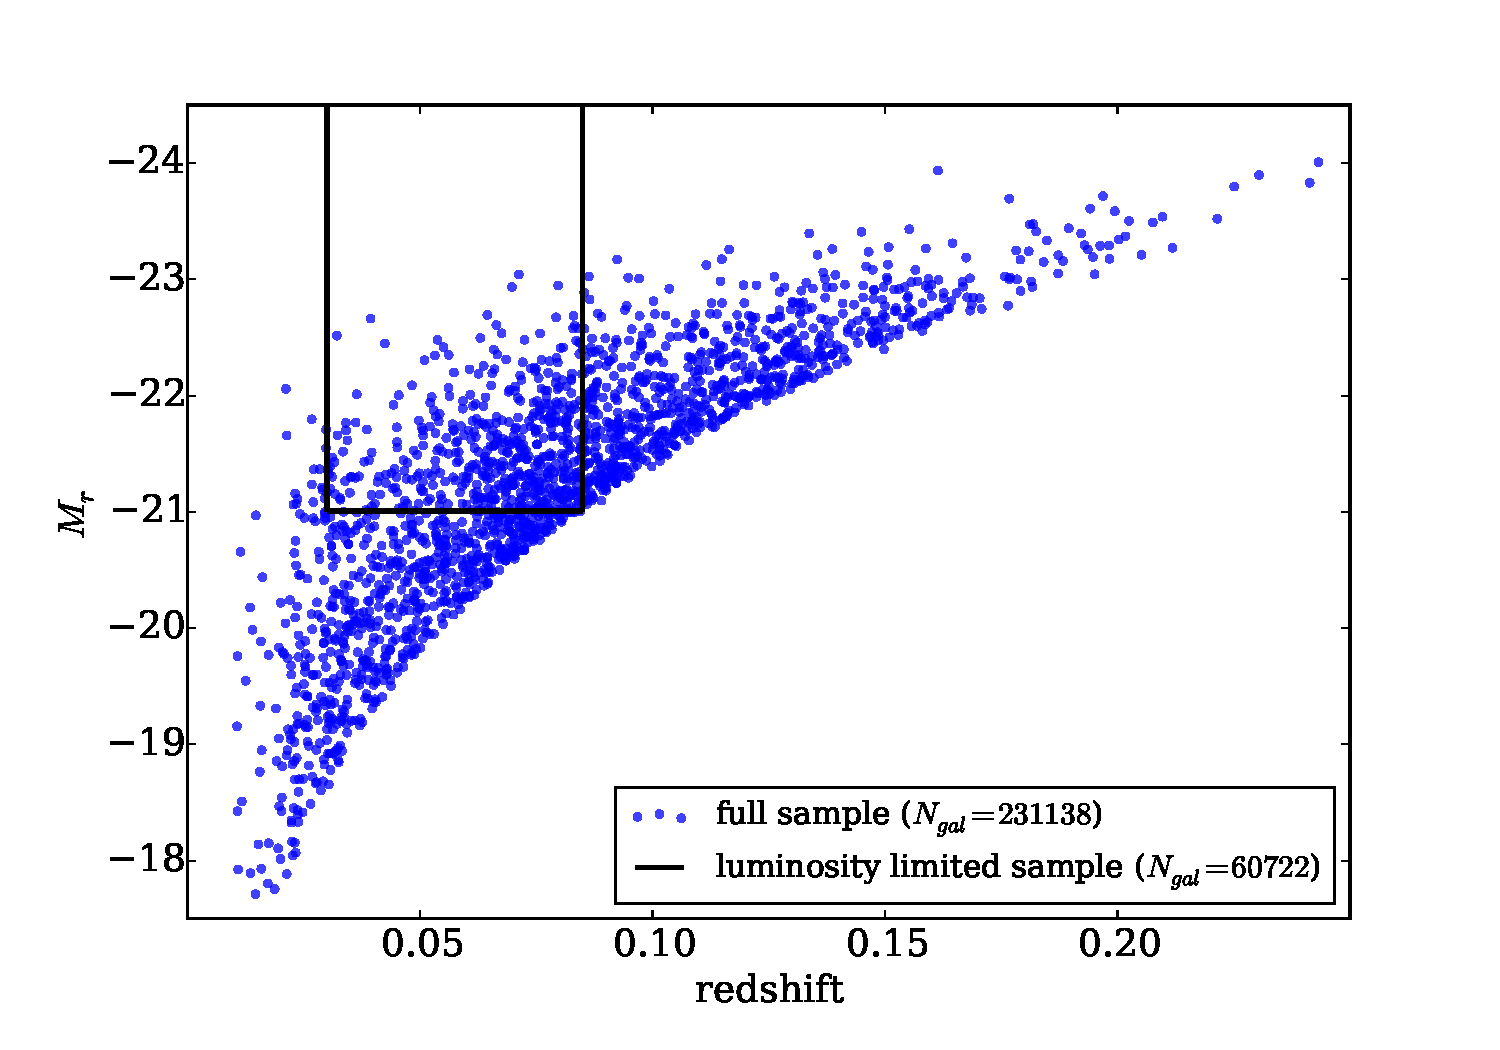
\includegraphics[width=0.5\textwidth]{Data_imgs/volume_limited_sample.pdf}
		
        \caption{Plot indicating the \textit{full sample} (red points) and the $0.03<z<0.085$ \textit{luminosity limited sample} (region enclosed within the black lines).}
		
        \label{fig:vl_sample}
        
\end{figure}



As there is a relation between absolute magnitude and galaxy colour \citep{Baldry_06}, a stellar mass limited sample is defined. The volume-limited sample is incomplete for red galaxies with $\log (M/M_{\odot}) < 10.6$. We therefore consider a further reduced sample of galaxies with $\log (M/M_{\odot}) \gtrsim 10.6$. The sample is complete for stellar mass above this limit and $M_r<-21.04$. This sample is referred to as the \textit{stellar mass limited sample}.

%------------------------------------------------------------------------------------
%%%%%%%%%%%%%%%%%%%%%%%%%%%%%%%%%%%%%%%%%%%%%%%%%%%%%%%%%%%%%%%%%%%%%%%%%%%%%%%%%%%%%
%------------------------------------------------------------------------------------

\section{Correcting for redshift bias}

\subsection{Different ways of quantifying morphology in Galaxy Zoo}

There are two distinct techniques of using Galaxy Zoo morphologies to look for trends of visual morphology with respect to other galaxy properties, such as environment, colour or stellar mass. The first technique involves using the vote fractions themselves to classify galaxies. This method involves looking for enhancements in overall vote fractions as an indicator of morphological change \citep{Bamford_09,Casteels_13,Willett_13}\rh{+loads of others}. However, we may also want to quantify morphology using a method where we divide our galaxies into separate subsamples. For example, galaxies could be separated in to separate samples of spirals and ellipticals, \citep{Skibba_09,Smethurst_15}, allowing us to compare the respective properties of different galaxy poulations against each other directly. It is this 'thresholding' technique that is the focus of the work in this paper.

\subsection{Biases in the Galaxy Zoo sample}

Without any evolution in the population of galaxies, the 'true' distribution of morphologies does not change. However, the apparent brightness and size of galaxies can change depending on the distance at which it is viewed \citep{Bamford_09}. The Galaxy Zoo 2 sample includes SDSS galaxies and only includes galaxies up to a redshift of $\sim 0.25$, which is shallow enough to justify that there is no evolution in the true galaxy morphologies in our sample \citep{Willett_13}. However, the sample is still susceptible to \textit{classification bias}, due to the effect of how the images are presented in Galaxy Zoo. Due to their distance, galaxies at high redshift appear fainter in the SDSS images than galaxies at lower redshift, and therefore have lower signal-to noise. This means that more detailed features may be more difficult to distinguish in galaxies at higher redshift. It should also be noted that such biases are not exclusive to Galaxy Zoo morphologies; difficulty in observing faint features in lower signal-to-noise galaxies is an inherent property of visual galaxy classifications. The advantage of using Galaxy Zoo classifications is that it gives us a statistical method of looking at Galaxy morphologies. As each of the galaxies in the full galaxy sample has been visually classified by a number of independent observers, we can model how the apparent presence of features evolves with redshift, and correct this bias accordingly.  \rh{Could maybe include a 'vf vs. z' diagram here to show the apparent evolution in morphology, as per my lunch talk?}

The effect of classification bias is an important property that must be corrected for if we want to compare morphologies using either of the two techniques mentioned above. An unbiased sample would be affected by defects in two ways. Firstly, samples for the most 'difficult to see' features would be incomplete, meaning that the samples may be affected by poor number statistics. The second issue that would affect the results is sample contamination. This means that samples of the 'easier to see' features would actually include several galaxies that have been mis-classified. Therefore, any differences in the properties of different sub-samples may be negated due to each of the samples actually being composed of several different types of galaxy that have been incorrectly assigned to a given galaxy type. 

\subsubsection{Previous attempt to correct for redshift bias}
\label{sec:previous_method}
\begin{figure}
		\centering
		
        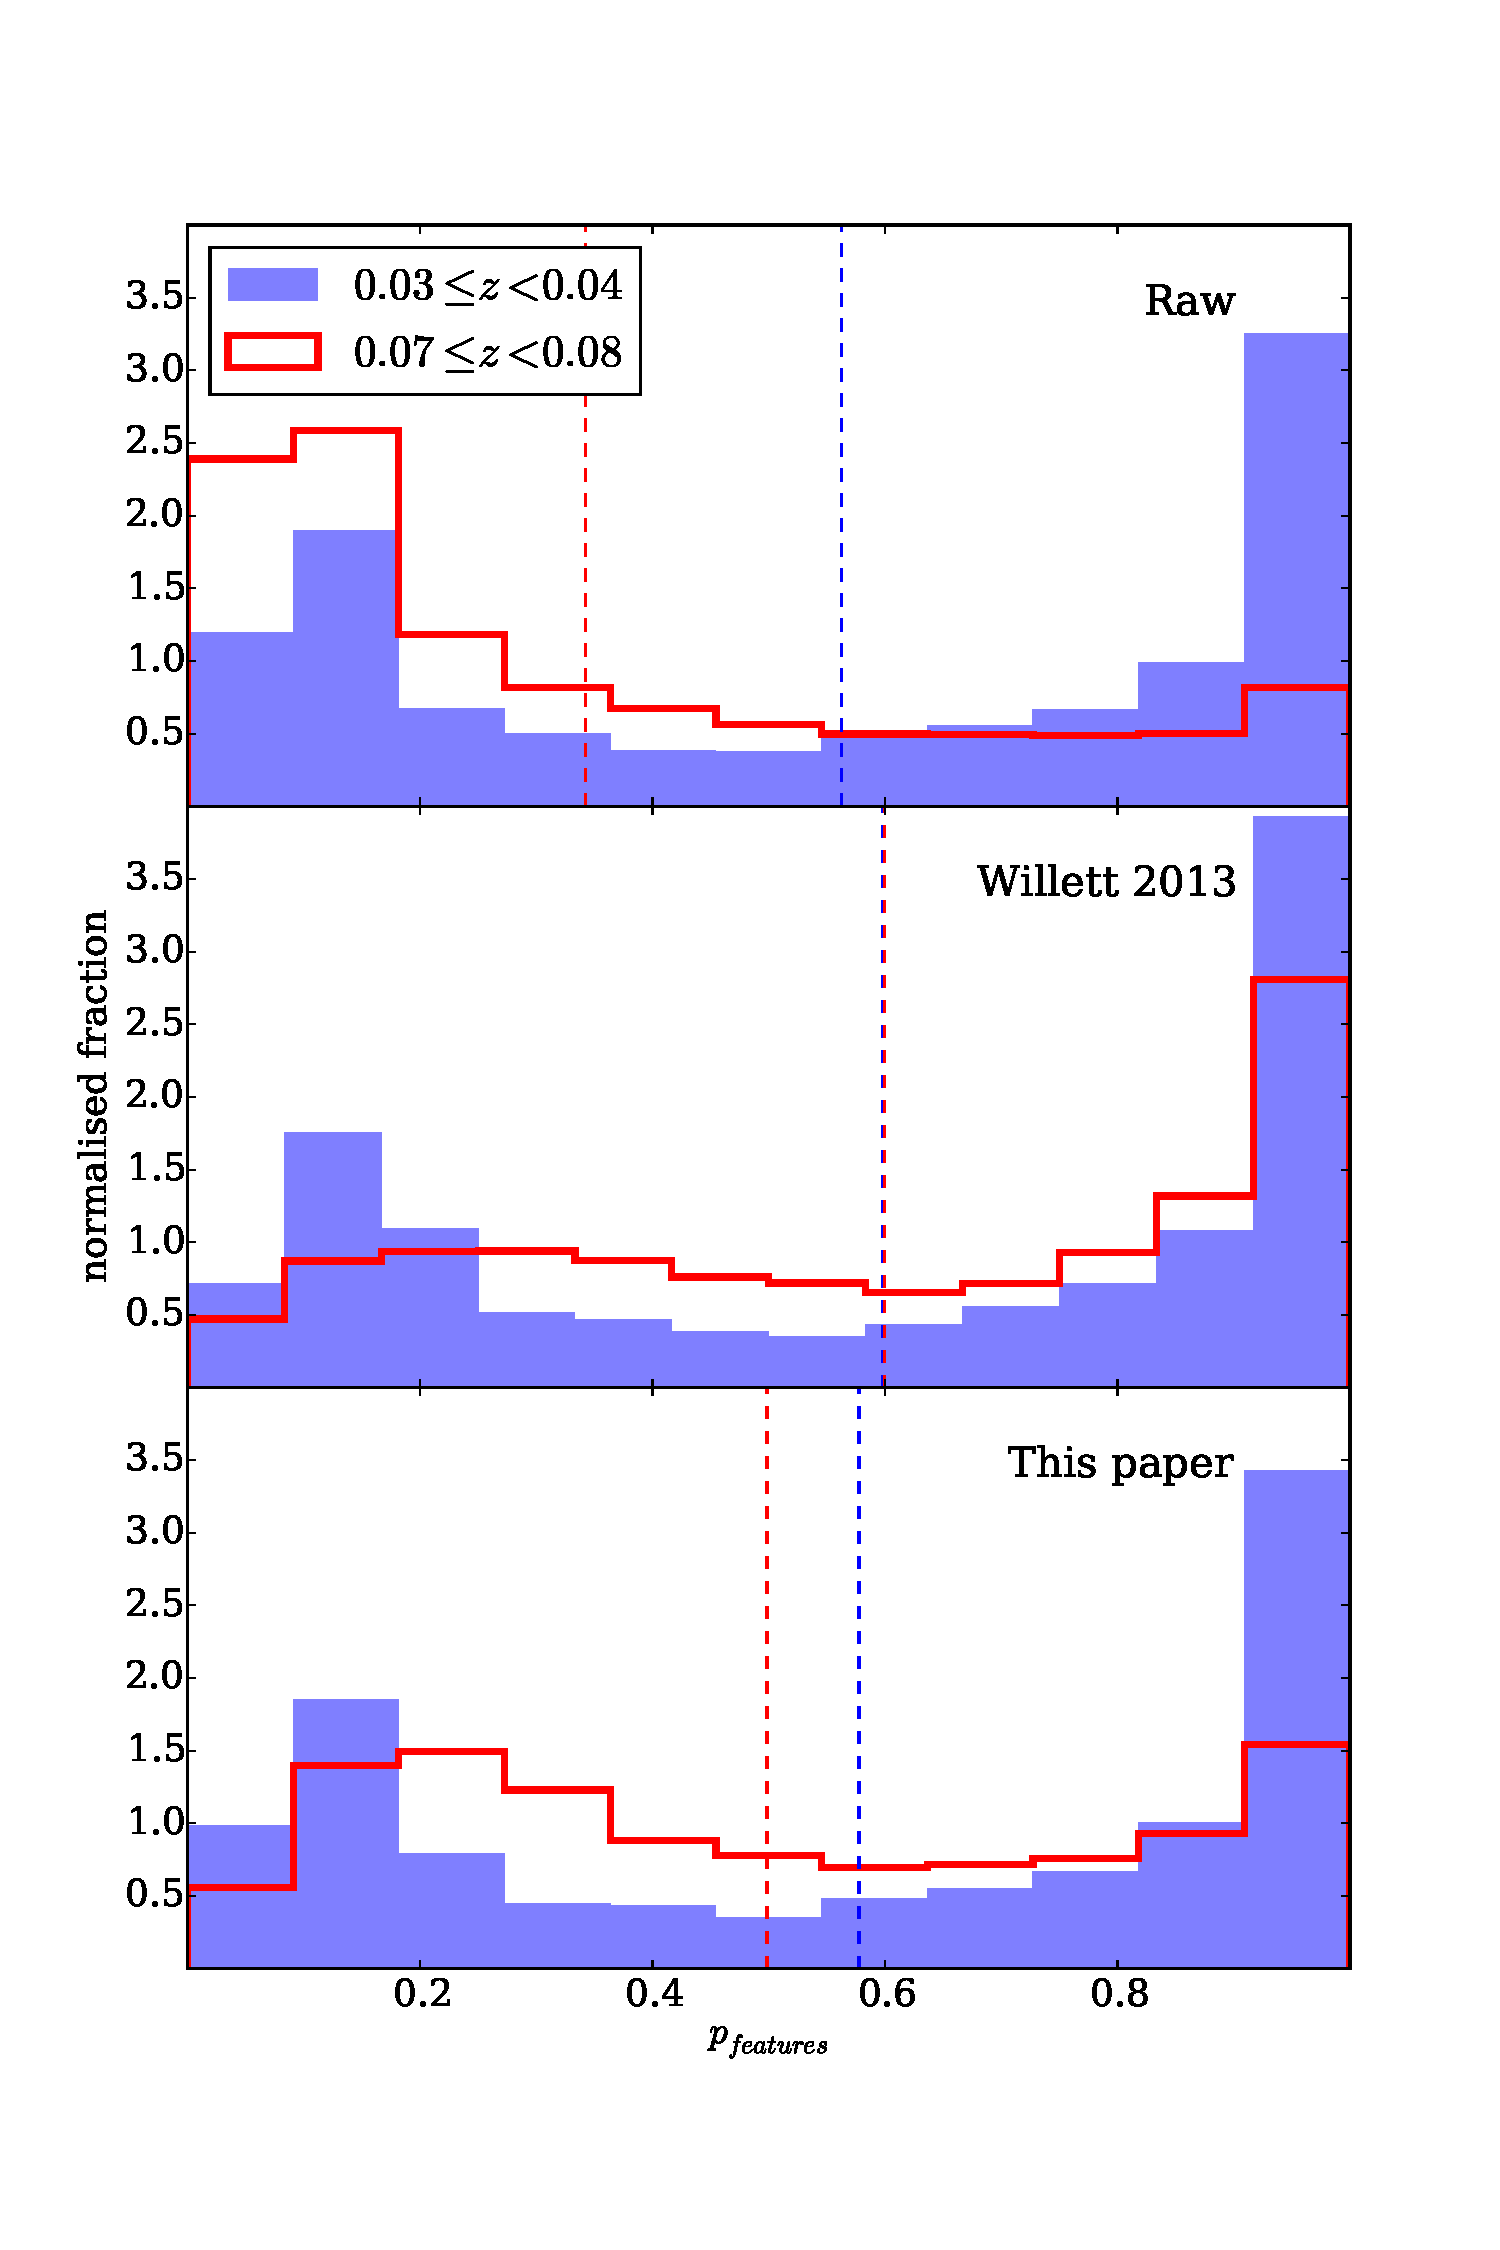
\includegraphics[width=0.5\textwidth]{Bias_imgs/vote_distribution_histograms.pdf}
		
        \caption{Distributions of answers to the 'features or disk' question of GZ2 for two different redshift ranges. The top panel indicates the raw vote distributions. The middle panel shows the distributions after debiasing using the method described in \citep{Willett_13} and the bottom panel shows the resulting distribution using the debiasing method described in this paper. The histogram bin widths are calculated according to the method described in \citet{Knuth_06} applied to the low redshift samples.}
		
        \label{fig:vote_histogram}
        
\end{figure}

The previous debiasing procedure applied to both Galaxy Zoo 1 (GZ1) and Galaxy Zoo 2 (GZ2) has focussed on adjusting the vote fractions of the galaxy samples by fixing the mean vote fractions as a function of redshift, a method first proposed in \citep{Bamford_09}. The method was updated for GZ2 in \citep{Willett_13}, with the key difference being that GZ2 has many non-binary questions. However, the limitations of this debiasing method are clear in figure \ref{fig:vote_histogram}, which shows the vote fraction distributions for the 'features or disk' answer to the first question in two different redshift bins. Although figure \ref{fig:vote_histogram} shows that the mean vote fraction is adequately debiased, the actual shapes of the distributions are not. This means that the fraction of galaxies that we have in our sample as a function of redshift is  dependent on the where we make the cut in the value of $p_{threshold}$. 

\begin{figure*}
		\centering
		
        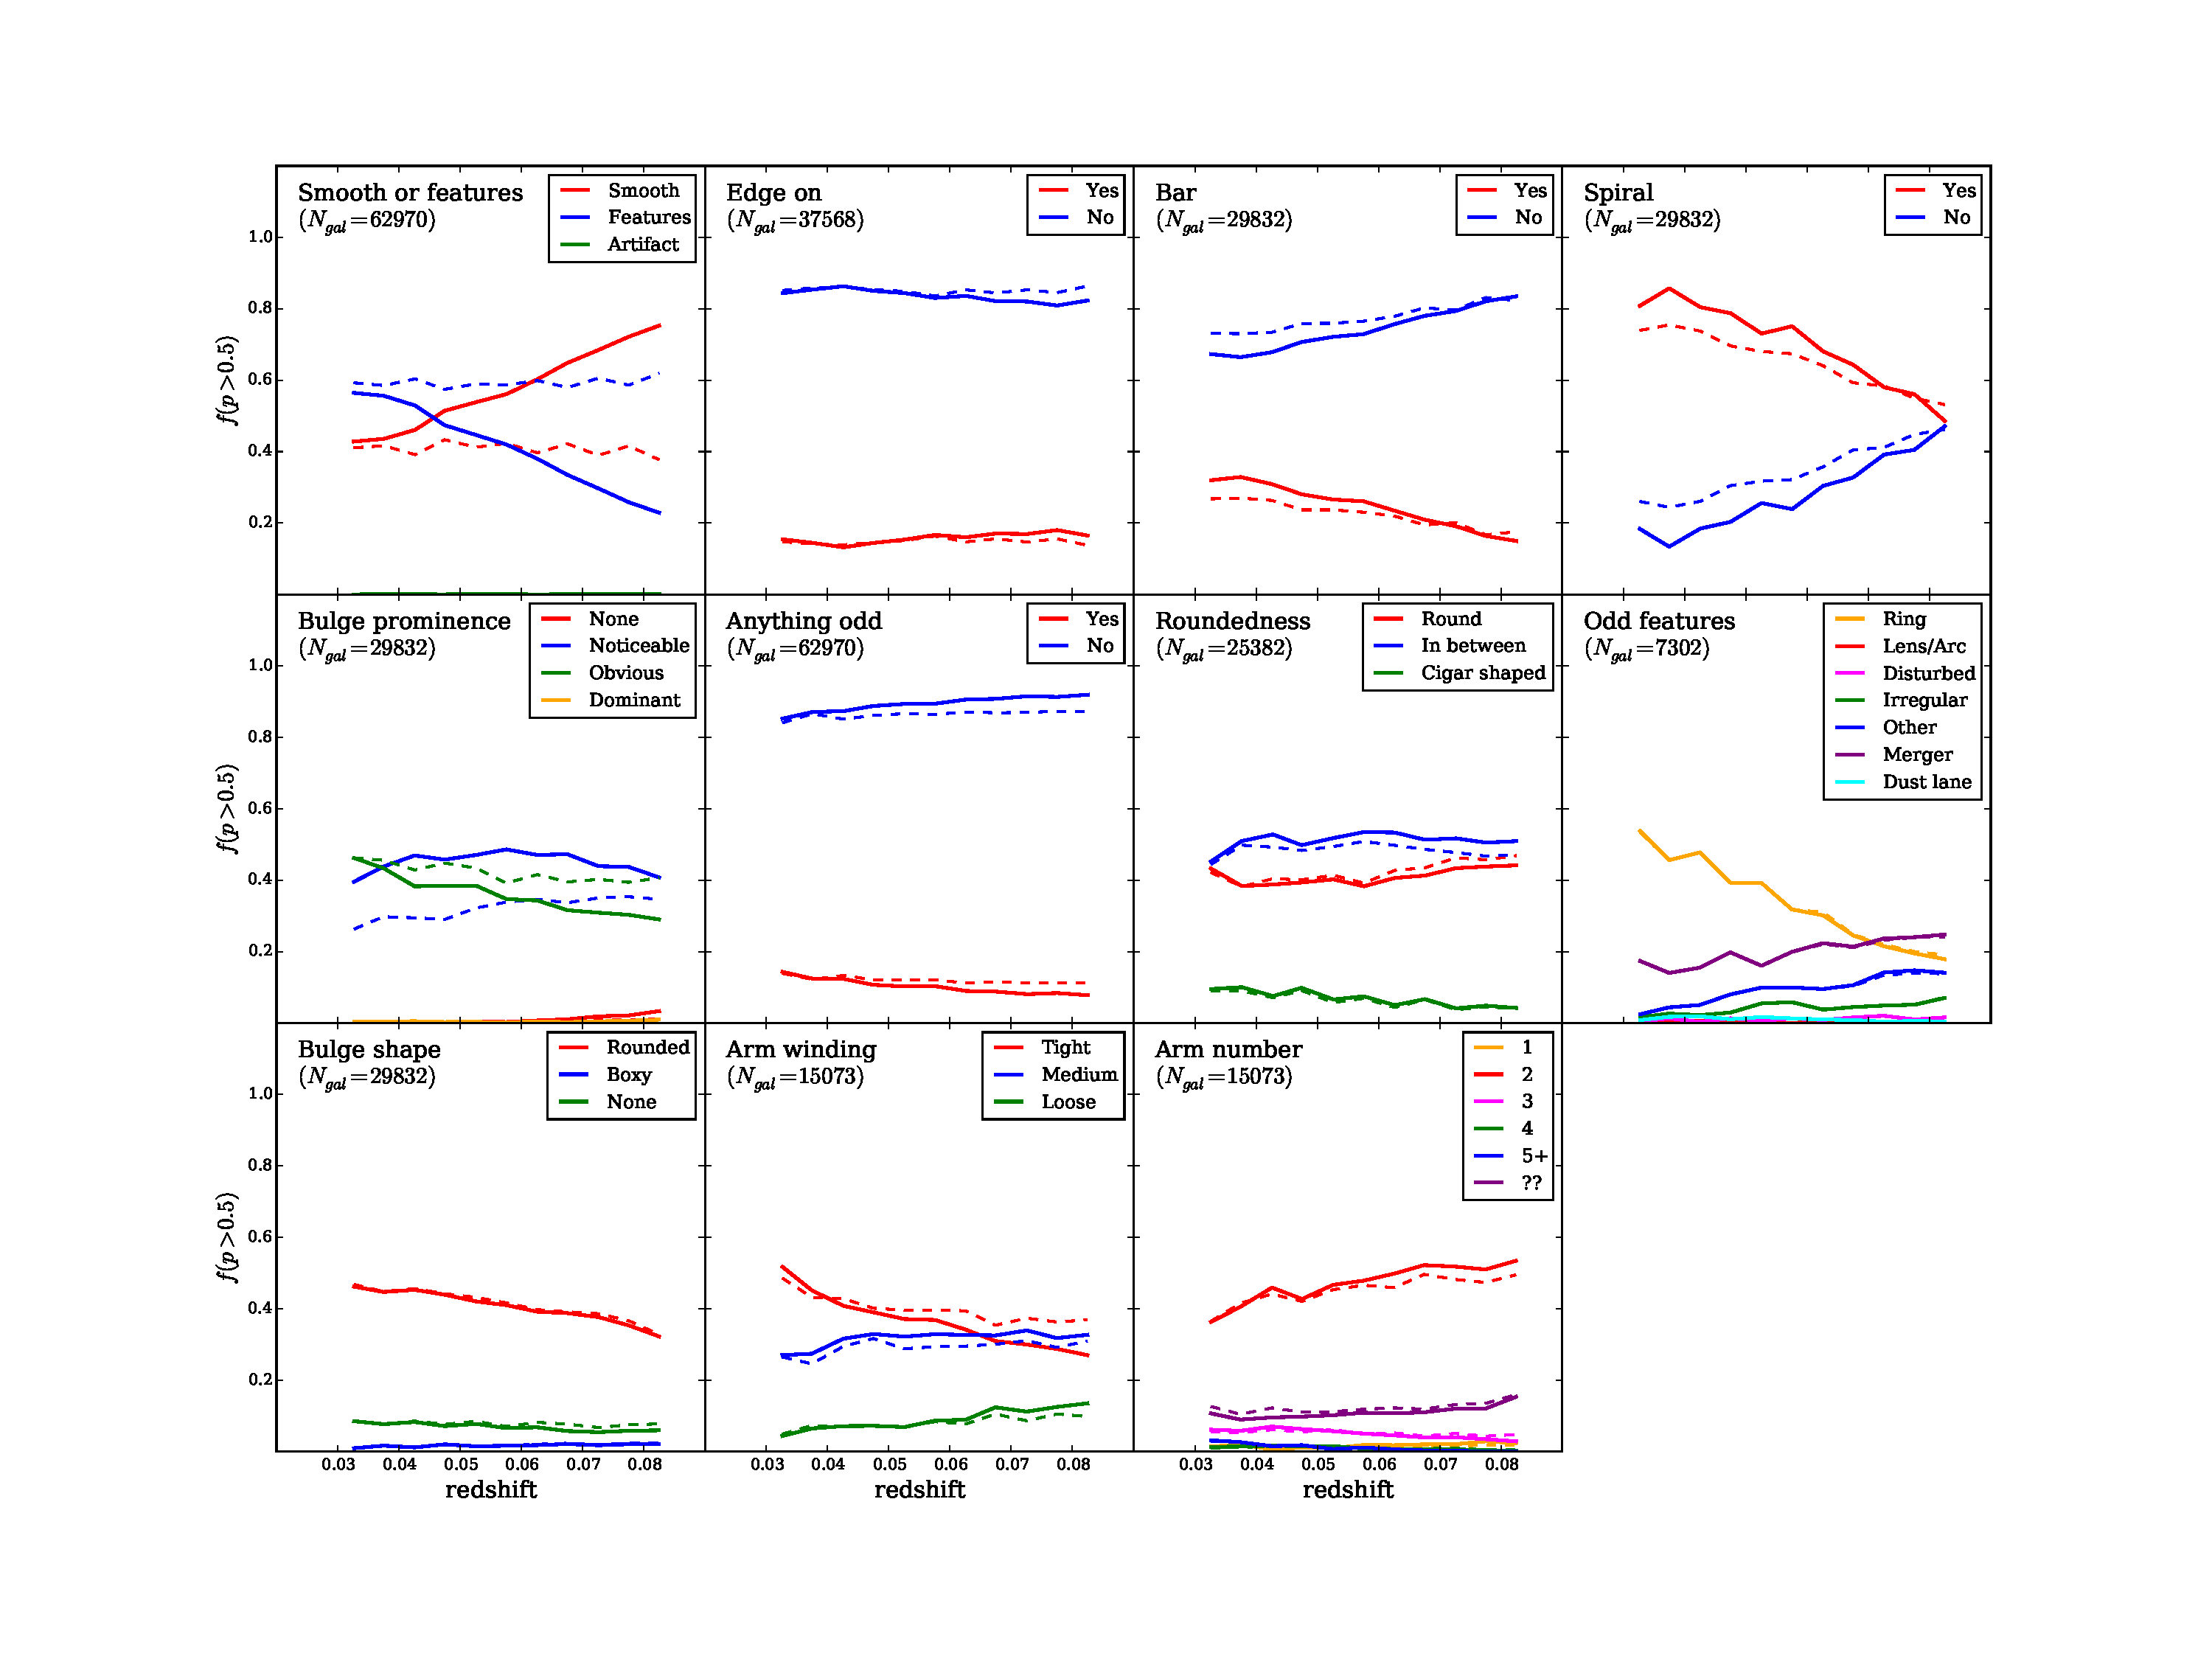
\includegraphics[width=1\textwidth]{Bias_imgs/vote_panel_plot.pdf}
		
        \caption{Fraction of galaxies with $p>0.5$ for each of the questions in GZ2. The solid lines indicate the raw vote fractions, and eh dashed lines indicate the debiased vote fractions from \citep{Willett_13}. Each sample is made up of only the galaxies in which more than half of the total classifiers answered that particular question.}
		
        \label{fig:vote_panel}
        
\end{figure*}

Further evidence that a new debiasing procedure is required is provided when we look at how the number of galaxies above a given threshold changes for each question. Figure \ref{fig:vote_panel} shows the fraction of galaxies in our \textit{luminosity limited sample} that have a particular feature as a function of redshift. An ideal debiasing procedure should keep the fractions in an inherently unbiased, \textit{luminosity limited sample} constant with redshift. Figure \ref{fig:vote_panel} shows that this is not the case for all of the questions in the sample. In figure \ref{fig:vote_panel} we define each of the samples of galaxies as all of the galaxies in which $p>0.5$ answered a particular question. For example, for the first 'features or disk' question, all of the galaxies are included in the sample, because every classification includes this question ($p=1$). However, for a user to say whether or not spiral arms are present, they must also have answered that they saw features, and that the disk was not edge-on. Therefore, we only include galaxies with $p_{features} \times p_{not ege on} > 0.5$, so the sample of galaxies is smaller. It is clear that making a threshold cut for some of the questions, such as the 'features or disk' question leaves us with complete 'smooth' and 'features' samples that have consistent fractions with redshift. However, it is also clear that this is not the case for all of the questions. In particular, we see a clear trend of losing galaxies at almost all redshifts with $p_{spiral} > 0.5$, leaving us with an incomplete sample of spiral galaxies if that particular threshold was chosen. Consequently, we require a new debiasing procedure to apply to the data if we wish to define a complete sample of spiral galaxies. 

\subsection{A new method for removing redshift bias}
\label{sec:new_method}

With the limitations described in section \ref{sec:previous_method}, we attempt to construct a new method of debiasing the GZ2 data more effectively. The new method aims to make the vote distributions themselves consistent with redshift rather than aiming for consistency in the mean vote fraction values. This debiasing method is made possible due to the number of individual classifications we have of each of the galaxies in our sample. As each galaxy is classified by 40 or more volunteers, we can attempt to model the evolution of the vote fractions as a function of redshift to make our samples as clean as possible. The main motivation behind this method is that different classifiers will have different levels of ability to pick out the most detailed features. Thus, as we go to higher redshift, where images have lower signal-to noise, we expect the overall vote fraction trend to also evolve, as some classifiers lose the ability to see the most detailed features. We aim to model this redshift bias by modelling the vote fraction histograms as a function of redshift, and correcting the higher redshift vote distributions to be as similar as possible to equivalent galaxies at low redshift. \rh{Terrible paragraph...}

\subsubsection{Binning the data by surface brightness}

\begin{figure}
		\centering
		
        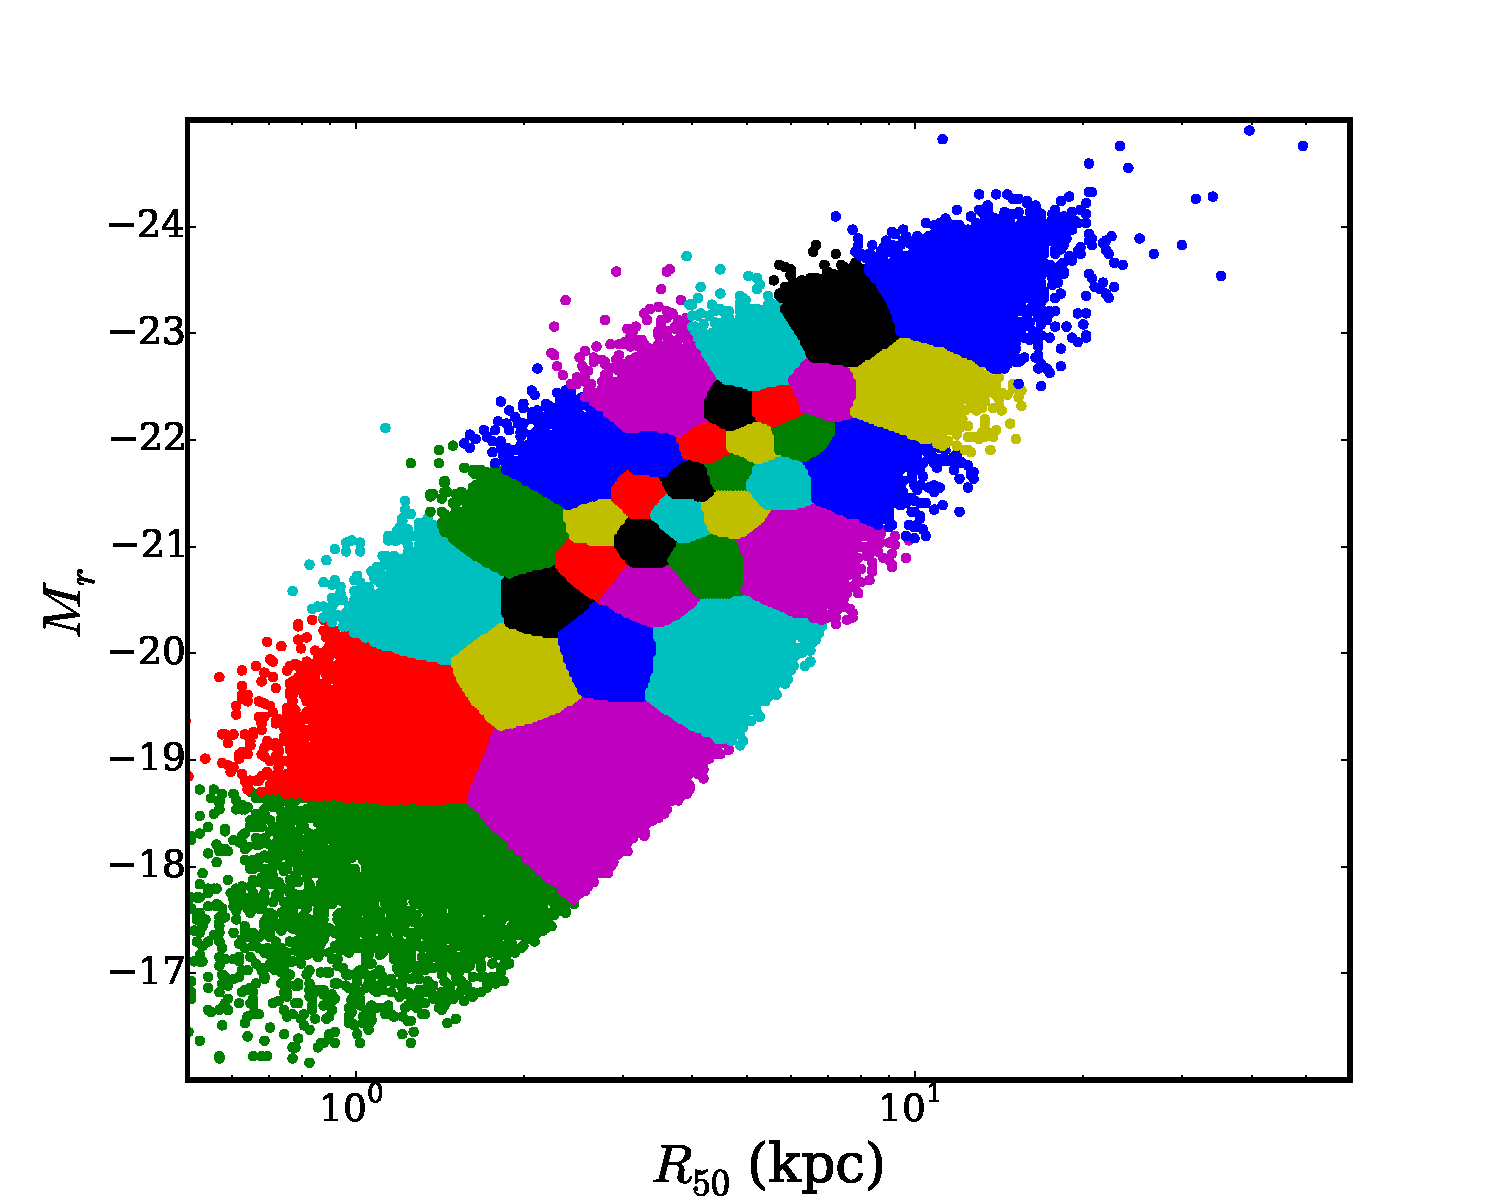
\includegraphics[width=0.5\textwidth]{Bias_imgs/voronoi_bins.pdf}
		
        \caption{Distribution of the voronoi bins in terms of $R_{50}$ and $M_r$. The bins were calculated using the method described in XX.} 
		
        \label{fig:voronoi_bins}
        
\end{figure}

To attempt to model the evolution of vote fractions, we first bin the data. We attempt to model galaxy properties as a function of three parameters- absolute magnitude, galaxy radius and redshift. It is imperative that intrinsic galaxy properties are accounted for, as there is expected to be an evolution in galaxy properties with different sizes and luminosities. To do this, we firstly bin the \textit{full sample} in terms of surface brightness, to model the change in vote fraction as a function of overall galaxy properties. We therefore voronoi tesselate \rh{(cite?)} the data in terms of $\log(R_{50)}$ and $M_r$, with the aim of including $>5000$ galaxies in each of the voronoi bins. This generated 35 voronoi bins overall, with a mean value of 7110 galaxies per bin and a standard deviation of 1048 galaxies per bin. Bin 28 was the only bin that did not include $>5000$ galaxies, including only 3506 galaxies. The voronoi bins are shown in figure \ref{fig:voronoi_bins}. 

\subsubsection{Modelling redshift bias}

Having divided the sample in to different bins to allow us to model for intrinsic galaxy properties, we can now attempt to correct for the apparent evolution induced by classification bias as a function of redshift. For each of the questions in turn, we define a sample of galaxies to debias the data. To do this we select a sample of galaxies with $p>0.5$ of the debiased vote fraction having answered that question. For example, for an individual user to have answered the arm number question, they would have had to have said that a galaxy has features, is not edge on, and has spiral arms. To define a spiral sample of galaxies which are to be classified by arm number, we therefore impose a cut of $p_{features} \times p_{not \, edge \, on} \times p_{spiral} > 0.5$. We also impose a further cut to account for low signal. We use a value of $N \geq 5$ to ensure that at least 5 different individuals have answered the arm number question. This sample is used as the 'control' population to debias the data for a particular question.

It is vital that we keep a good level of 'signal' in each of the redshift bins. To account for this, we choose the bins adaptively depending on the answer to be debiased. For a given answer we select only the galaxies that have at least 1 vote ($p>0$), and then divide this sample in to different redshift bins. We aim to have $>50$ galaxies with $p>0$ for each bin, unless there are fewer than 3 redshift bins for a given voronoi bin- in that case we sacrifice a higher 'signal' and divide that particular voronoi bin in to 5 redshift bins, to allow us to model the 'evolution' in the vote fraction distribution as a function of redshift. \rh{Can we do a 'weighting' to improve this?}

After dividing the sample in to different redshift bins for each of the voronoi bins, we now fit functions to model the data. To do this, we model the data in terms of $\log(f_v)$, where $f_v$ is the vote fraction for a given question vs. the cumulative fraction. Modelling the cumulative histograms in $\log$ space effectively stretches out the histogram at the lowest end ($f_v \approx 0$). This is particularly useful for the questions where the vote fractions are split between multiple categories, such as the question about the number of spiral arms, as most of the votes are concentrated at $f_v \approx 0$. For each of the redshift bins in turn, and each of the voronoi bins in turn, a cumulative histogram is plotted and a function is fit to model the shape of that particular histogram. We have selected three different functions to model each of the histograms: a logistic function (equation 1) , an exponential power function (equation 2) and an inverse x function (equation 3). The respective equations are listed below:

\begin{center}
$f(x) = \frac{L}{1+e^{-k(x-c)}} \, [1]$
\end{center}

\begin{center}
$f(x) = e^{kx^{c}} \, [2]$
\end{center}

\begin{center}
$f(x) = \frac{1}{1 + k(-x)^c} \, [3]$
\end{center}

where k and c parameterise the shape of each of the curves. We fix the $L$ term with respect to $c$ in the logistic function so that any curve passes through the point $(0,1)$, corresponding to a cumulative fraction of $1$ when $f_v = 1$. Each of the functions passes through $(-\infty,0)$ and $(0,1)$, meaning that there is a single cumulative fraction that corresponds to each of the possible values of $0 \leq f_v \leq 1$. A single function is chosen to fit to all of the individual answers, by fitting each of the functions to the total data for each answer, and selecting the function which has the lowest $\chi^2$ value as calculated using the Python $scipy.optimize.minimize$ package. 

After selecting a function, the function is fit to each of the redshift bins for each of the voronoi bins, calculating optimal $k$ and $c$ values. After calculating a $k$ and $c$ value for each of the bins, a linear function is applied to parameterise how $k$ and $c$ vary with $R_{50}$, $M_r$ and $z$, by fitting a linear function of the following form:

\begin{center}
$x = k_1M_r + k_2R_{50} +k_3z + k_4 \, [4]$
\end{center}

where $k_1$,$k_2$,$k_3$ parameterise the change in $k$ or $c$ with respect to $M_r$, $R_{50}$ and $z$ respectively and $k_4$ is a constant. The $x$ value corresponds to the $k$ or $c$ value that parameterises the curve's shape. We use these values to estimate the shape of the cumulative histogram function for each galaxy with respect to its $R_{50}$, $M_r$ and $z$. We then use these values to correct the estimated histogram shape to its equivalent function at $z=0.03$, the lower redshift limit of the data. An example of the curves fit to the arm number answers is shown in figure \ref{fig:function_fit}. 

\begin{figure}
		\centering
		
        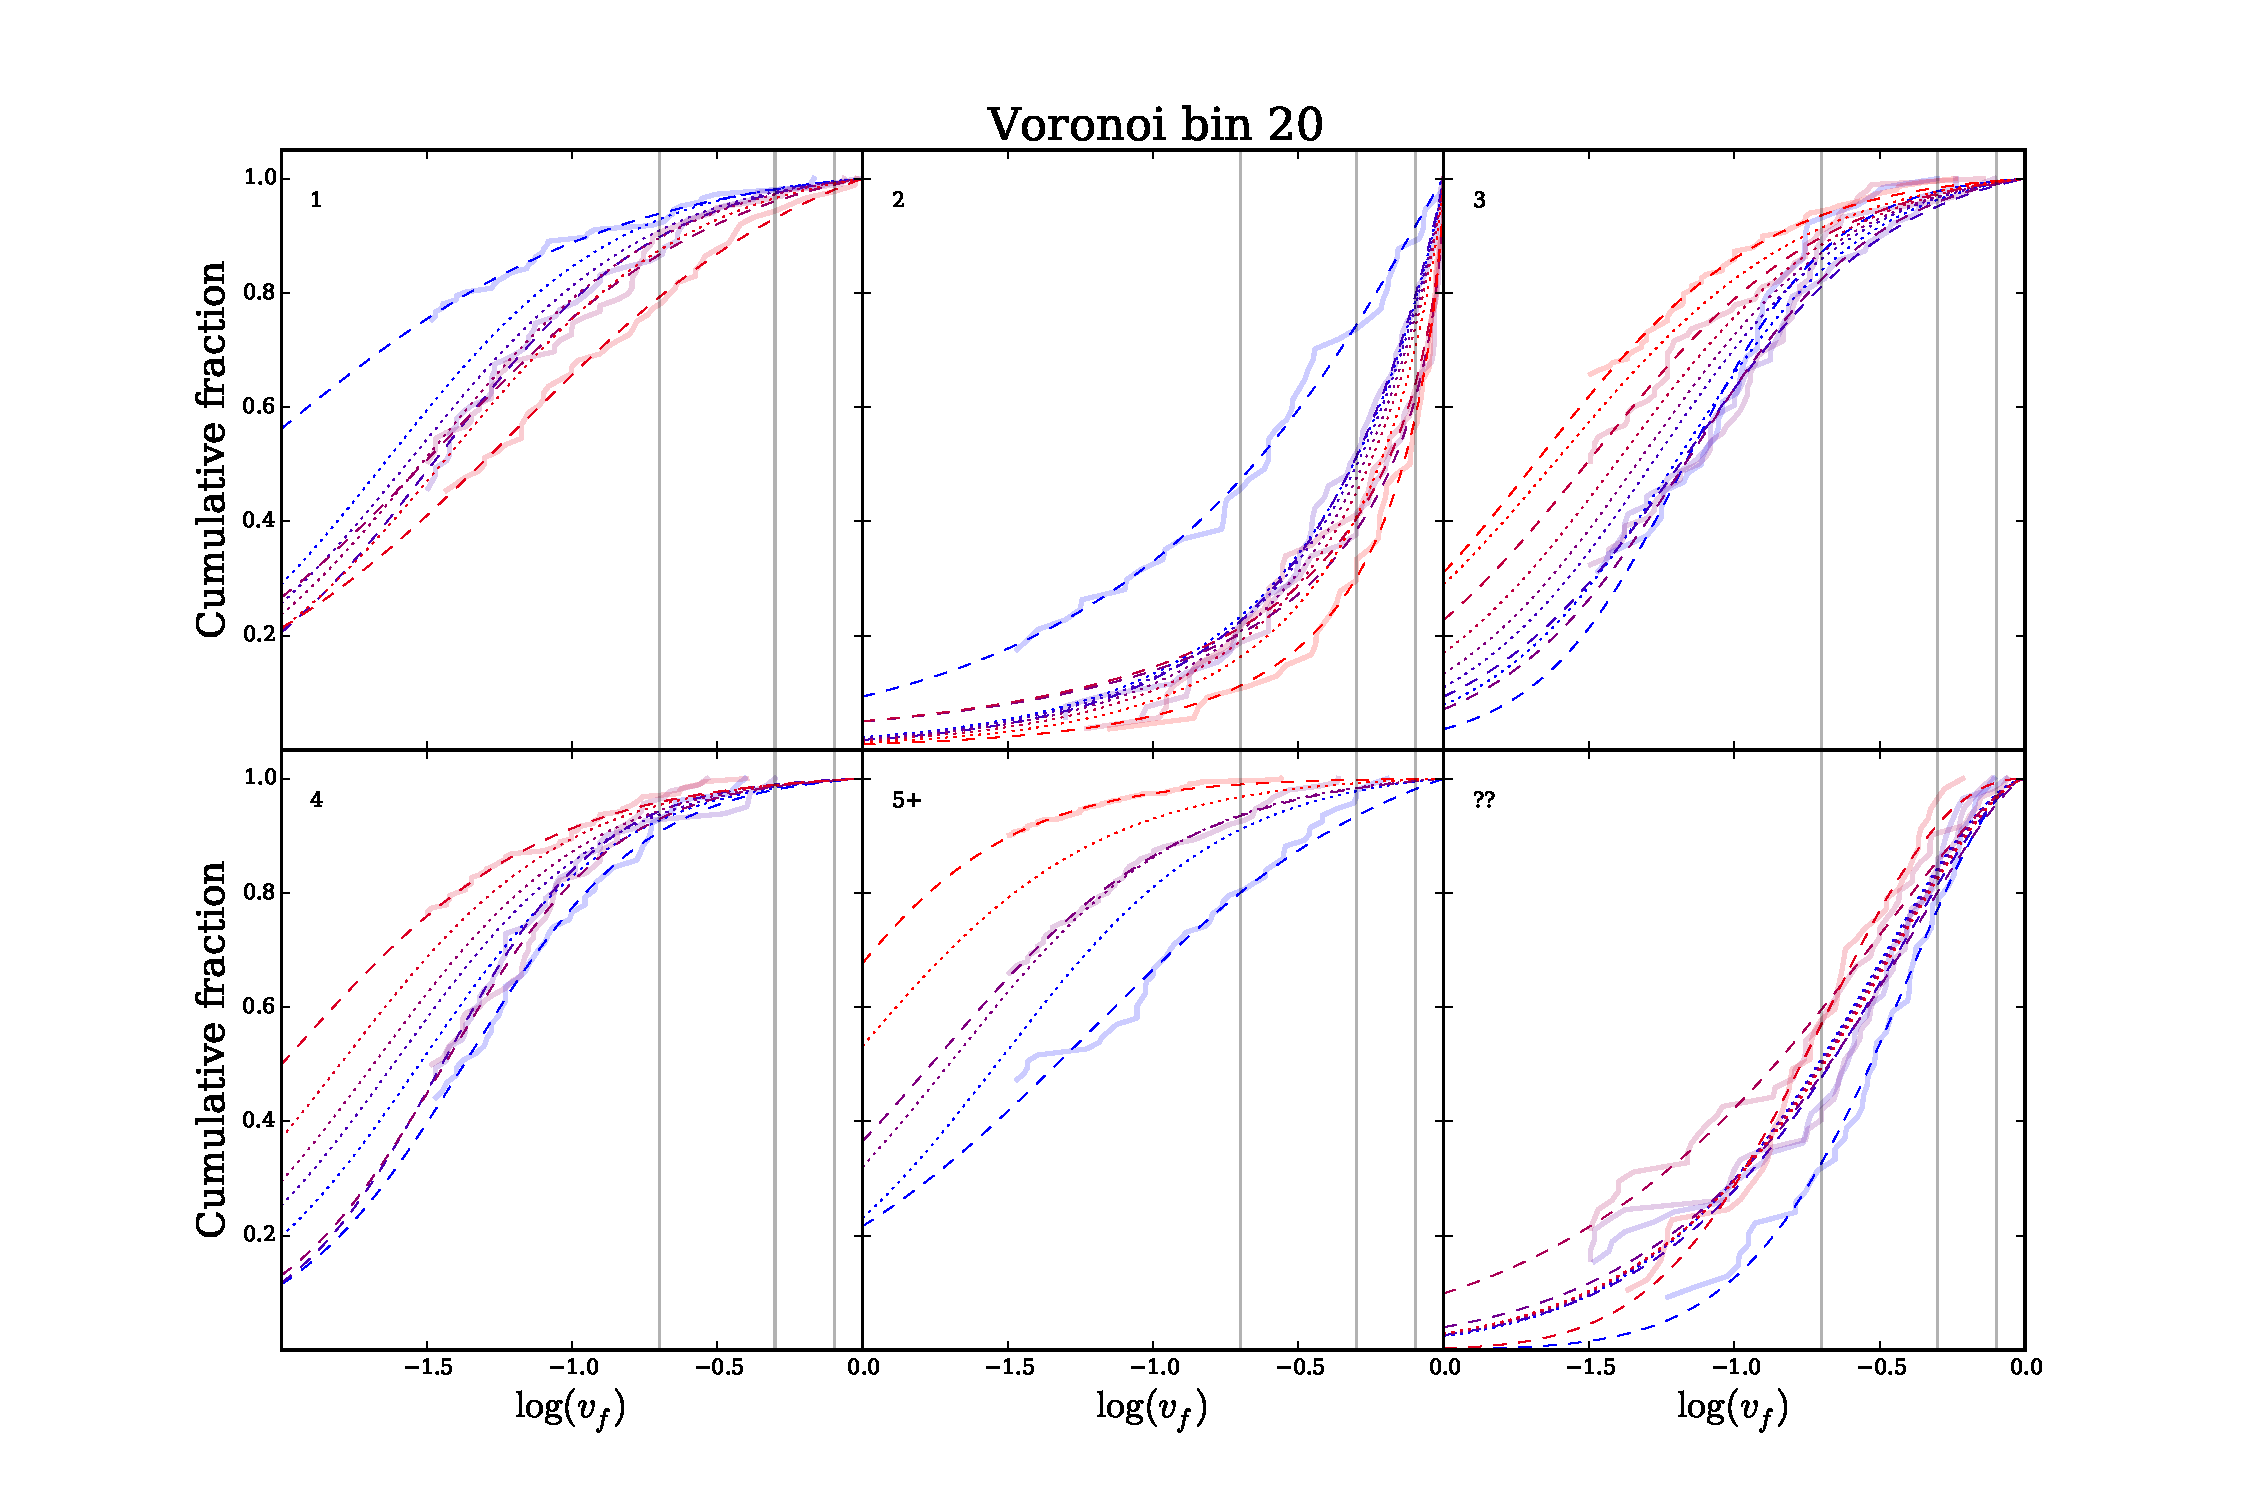
\includegraphics[width=0.5\textwidth]{Data_imgs/fit_t11_arms_number_vbin20_kcfit1.pdf}
		
        \caption{An example of a single voronoi bin fit for arm number. The red line indicates the highest redshift bin, and the blue line indicates the lowest redshift bin. The solid lines indicate the raw $f_v$ histograms, and the dashed lines show the best fit function to each of the corresponding histograms. The dotted lines show the corresponding approximation from the linear fit to the $k$ and $c$ values.}
		
        \label{fig:function_fit}
        
\end{figure}

\subsubsection{Results from the new debiasing method}

\begin{figure*}
		\centering
		
        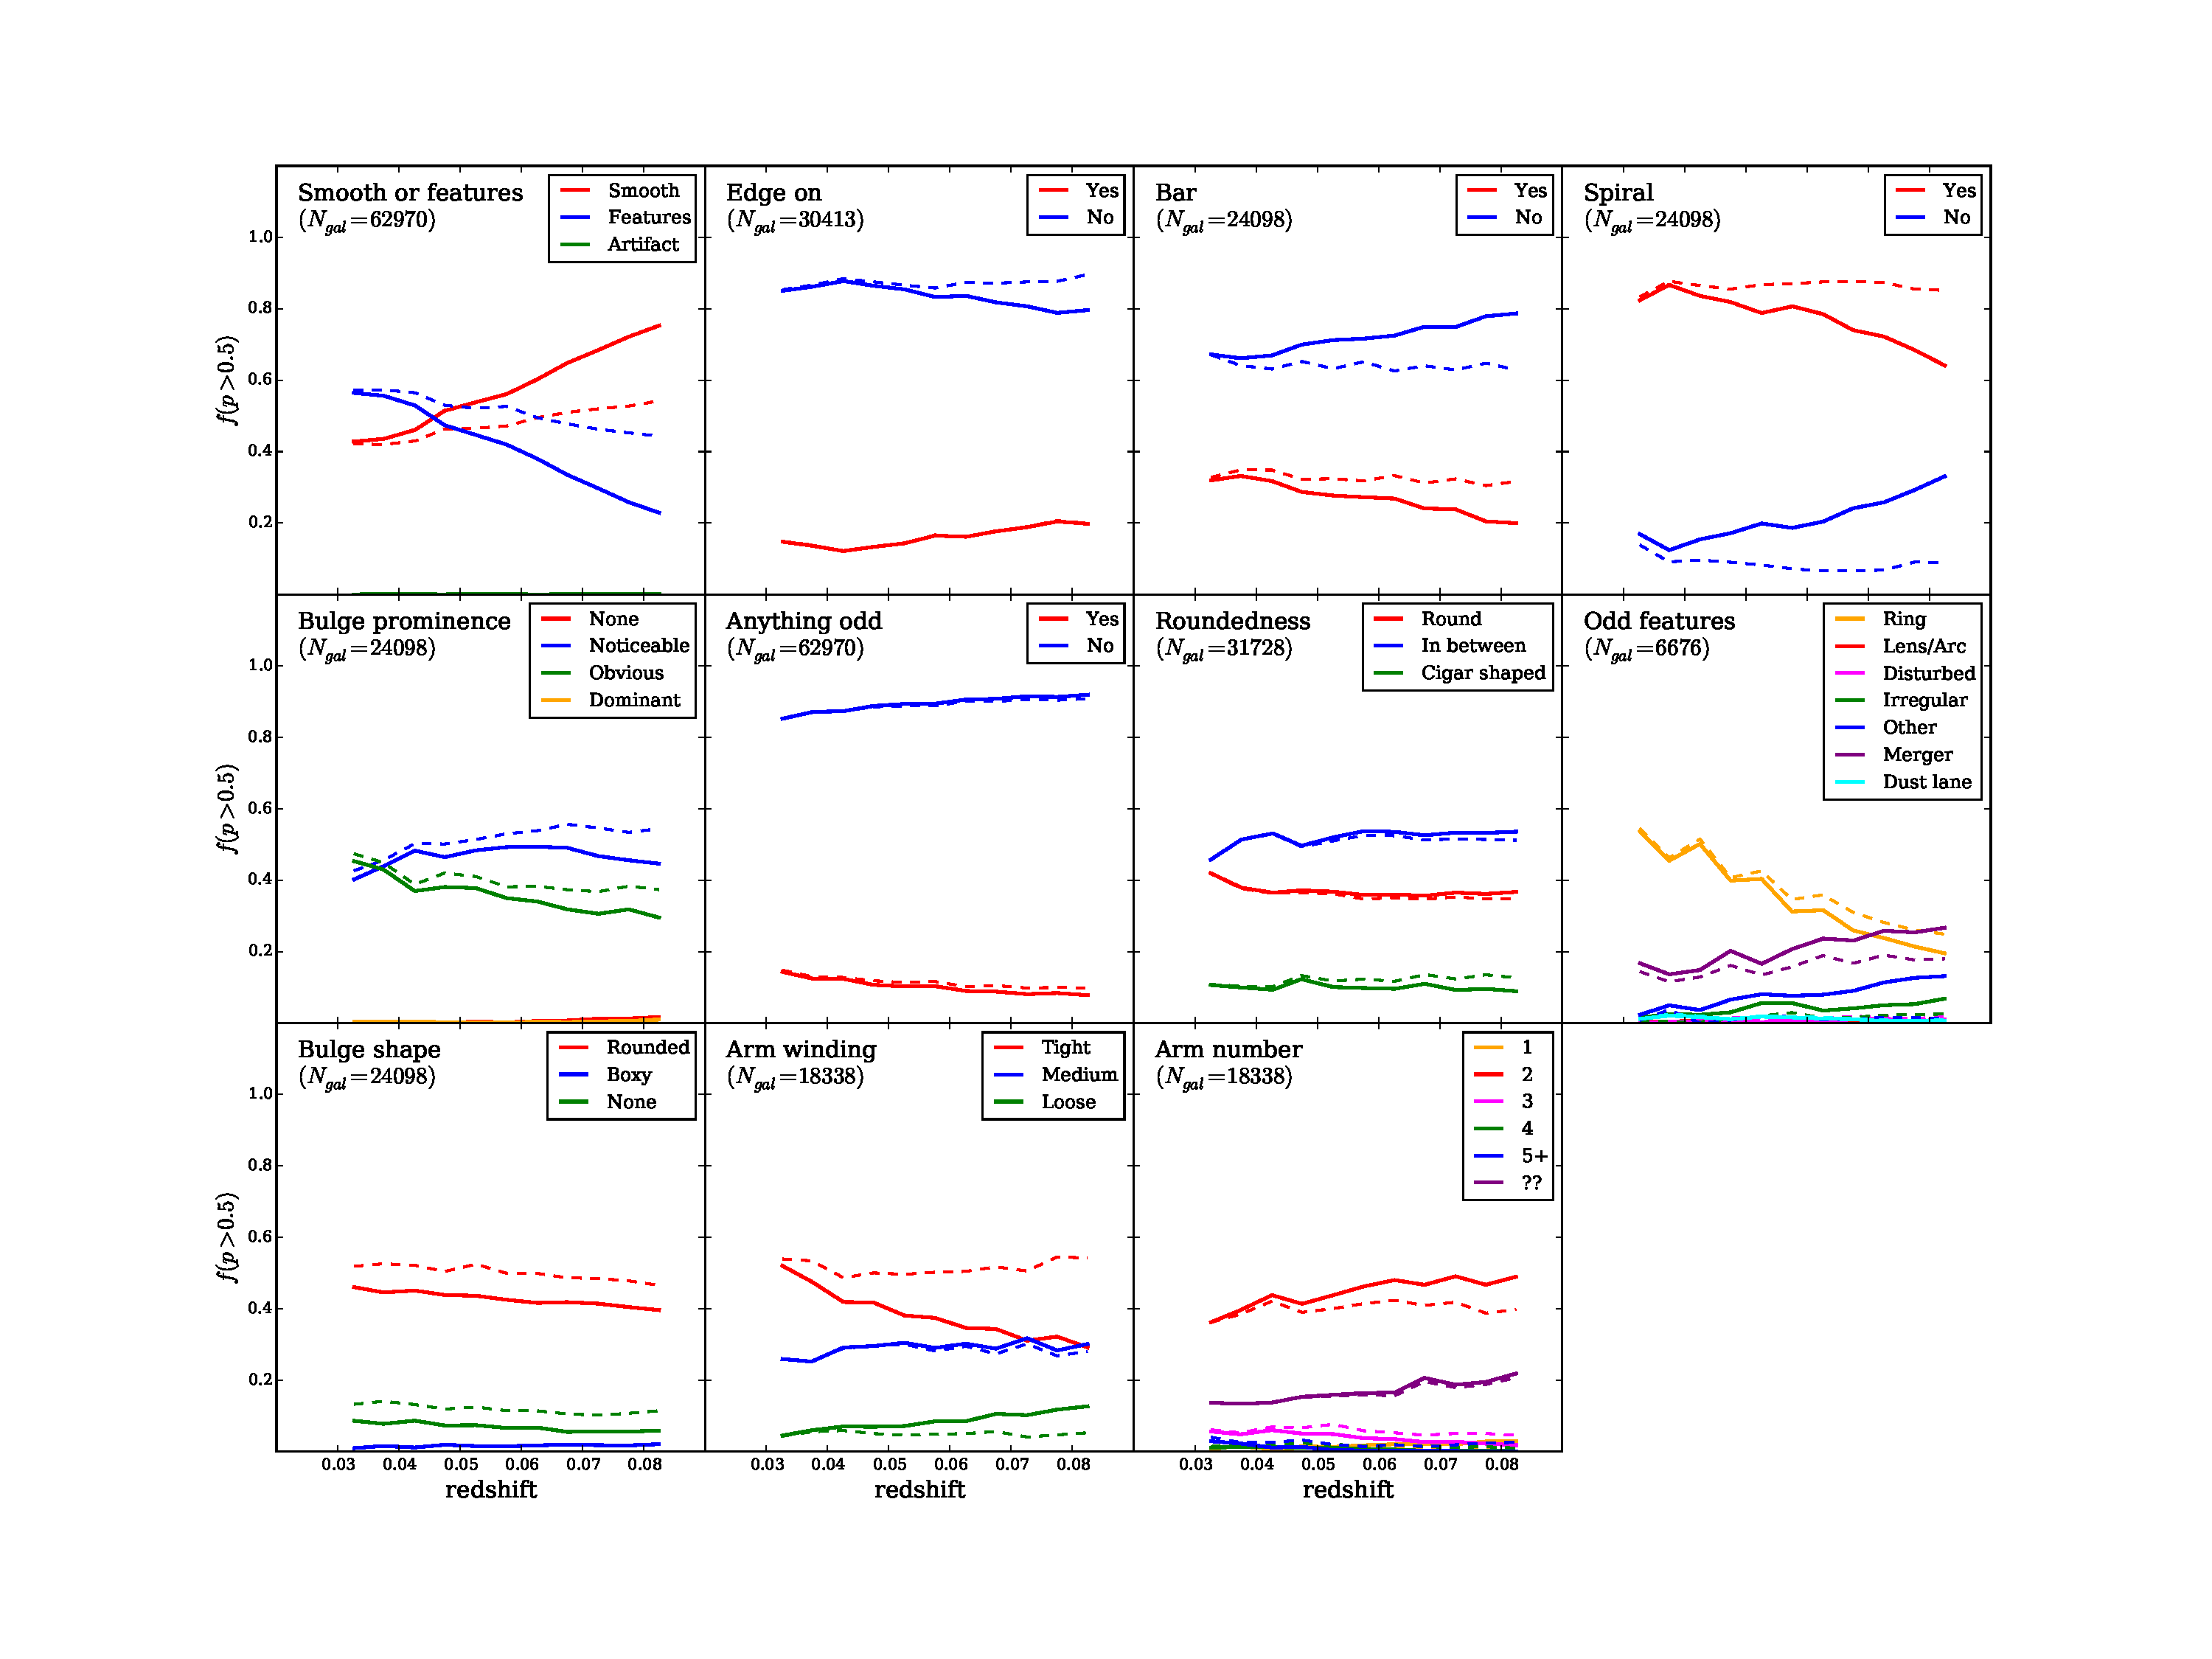
\includegraphics[width=1\textwidth]{Bias_imgs/vote_panel_plot_debiased.pdf}
		
        \caption{As in figure \ref{fig:vote_panel}, but using the debiasing procedure described in section \ref{sec:new_method}. The solid lines indicate the raw vote fractions, and the dashed lines indicate the debiased vote fractions. Each sample is made up of only the galaxies in which more than half of the total classifiers answered that particular question.\rh{N-cut???}}
		
        \label{fig:vote_panel_debiased}
        
\end{figure*}

Figure \ref{fig:vote_panel_debiased} shows the vote fractions as a function of redshift for the \textit{luminosity limited sample}. Such a sample should be spectroscopically complete at all redshifts, so we expect to see no evolution in galaxy properties with redshift in such a sample. Each of the samples is defined in the same way as described in section \ref{sec:previous_method}. The figures show that when we define samples by making selection cuts at $p>0.5$, the new debiasing procedure removes the apparent redshift evolution more consistently than the previous method employed in \citet{Willett_13}. In particular, we see that if we wish to define a spiral sample imposing a cut of $p_{features} \times p_{not \, edge \, on} \times p_{spiral} > 0.5$, to look in to spiral arm number, then the sample is more complete. It appears that the previous debiasing procedure did not debias the 'spiral' question effectively, with there being fewer spiral galaxies at higher redshift, as can be seen in the top right hand panel of figure \ref{fig:vote_panel}. In our debiasing procedure, we effectively 'flatten out' the fraction of gaalxies with $p_spiral>0.5$ with redshift, as can be seen from the top right hand panel of figure \ref{fig:vote_panel_debiased}. 


%------------------------------------------------------------------------------------
%%%%%%%%%%%%%%%%%%%%%%%%%%%%%%%%%%%%%%%%%%%%%%%%%%%%%%%%%%%%%%%%%%%%%%%%%%%%%%%%%%%%%
%------------------------------------------------------------------------------------
\section{Application to arm number}
\label{sec:results}

%------------------------------------------------------------------------------------

\subsection{Defining the sample}

\rh{Put table here}

\begin{figure}
		\centering
		
        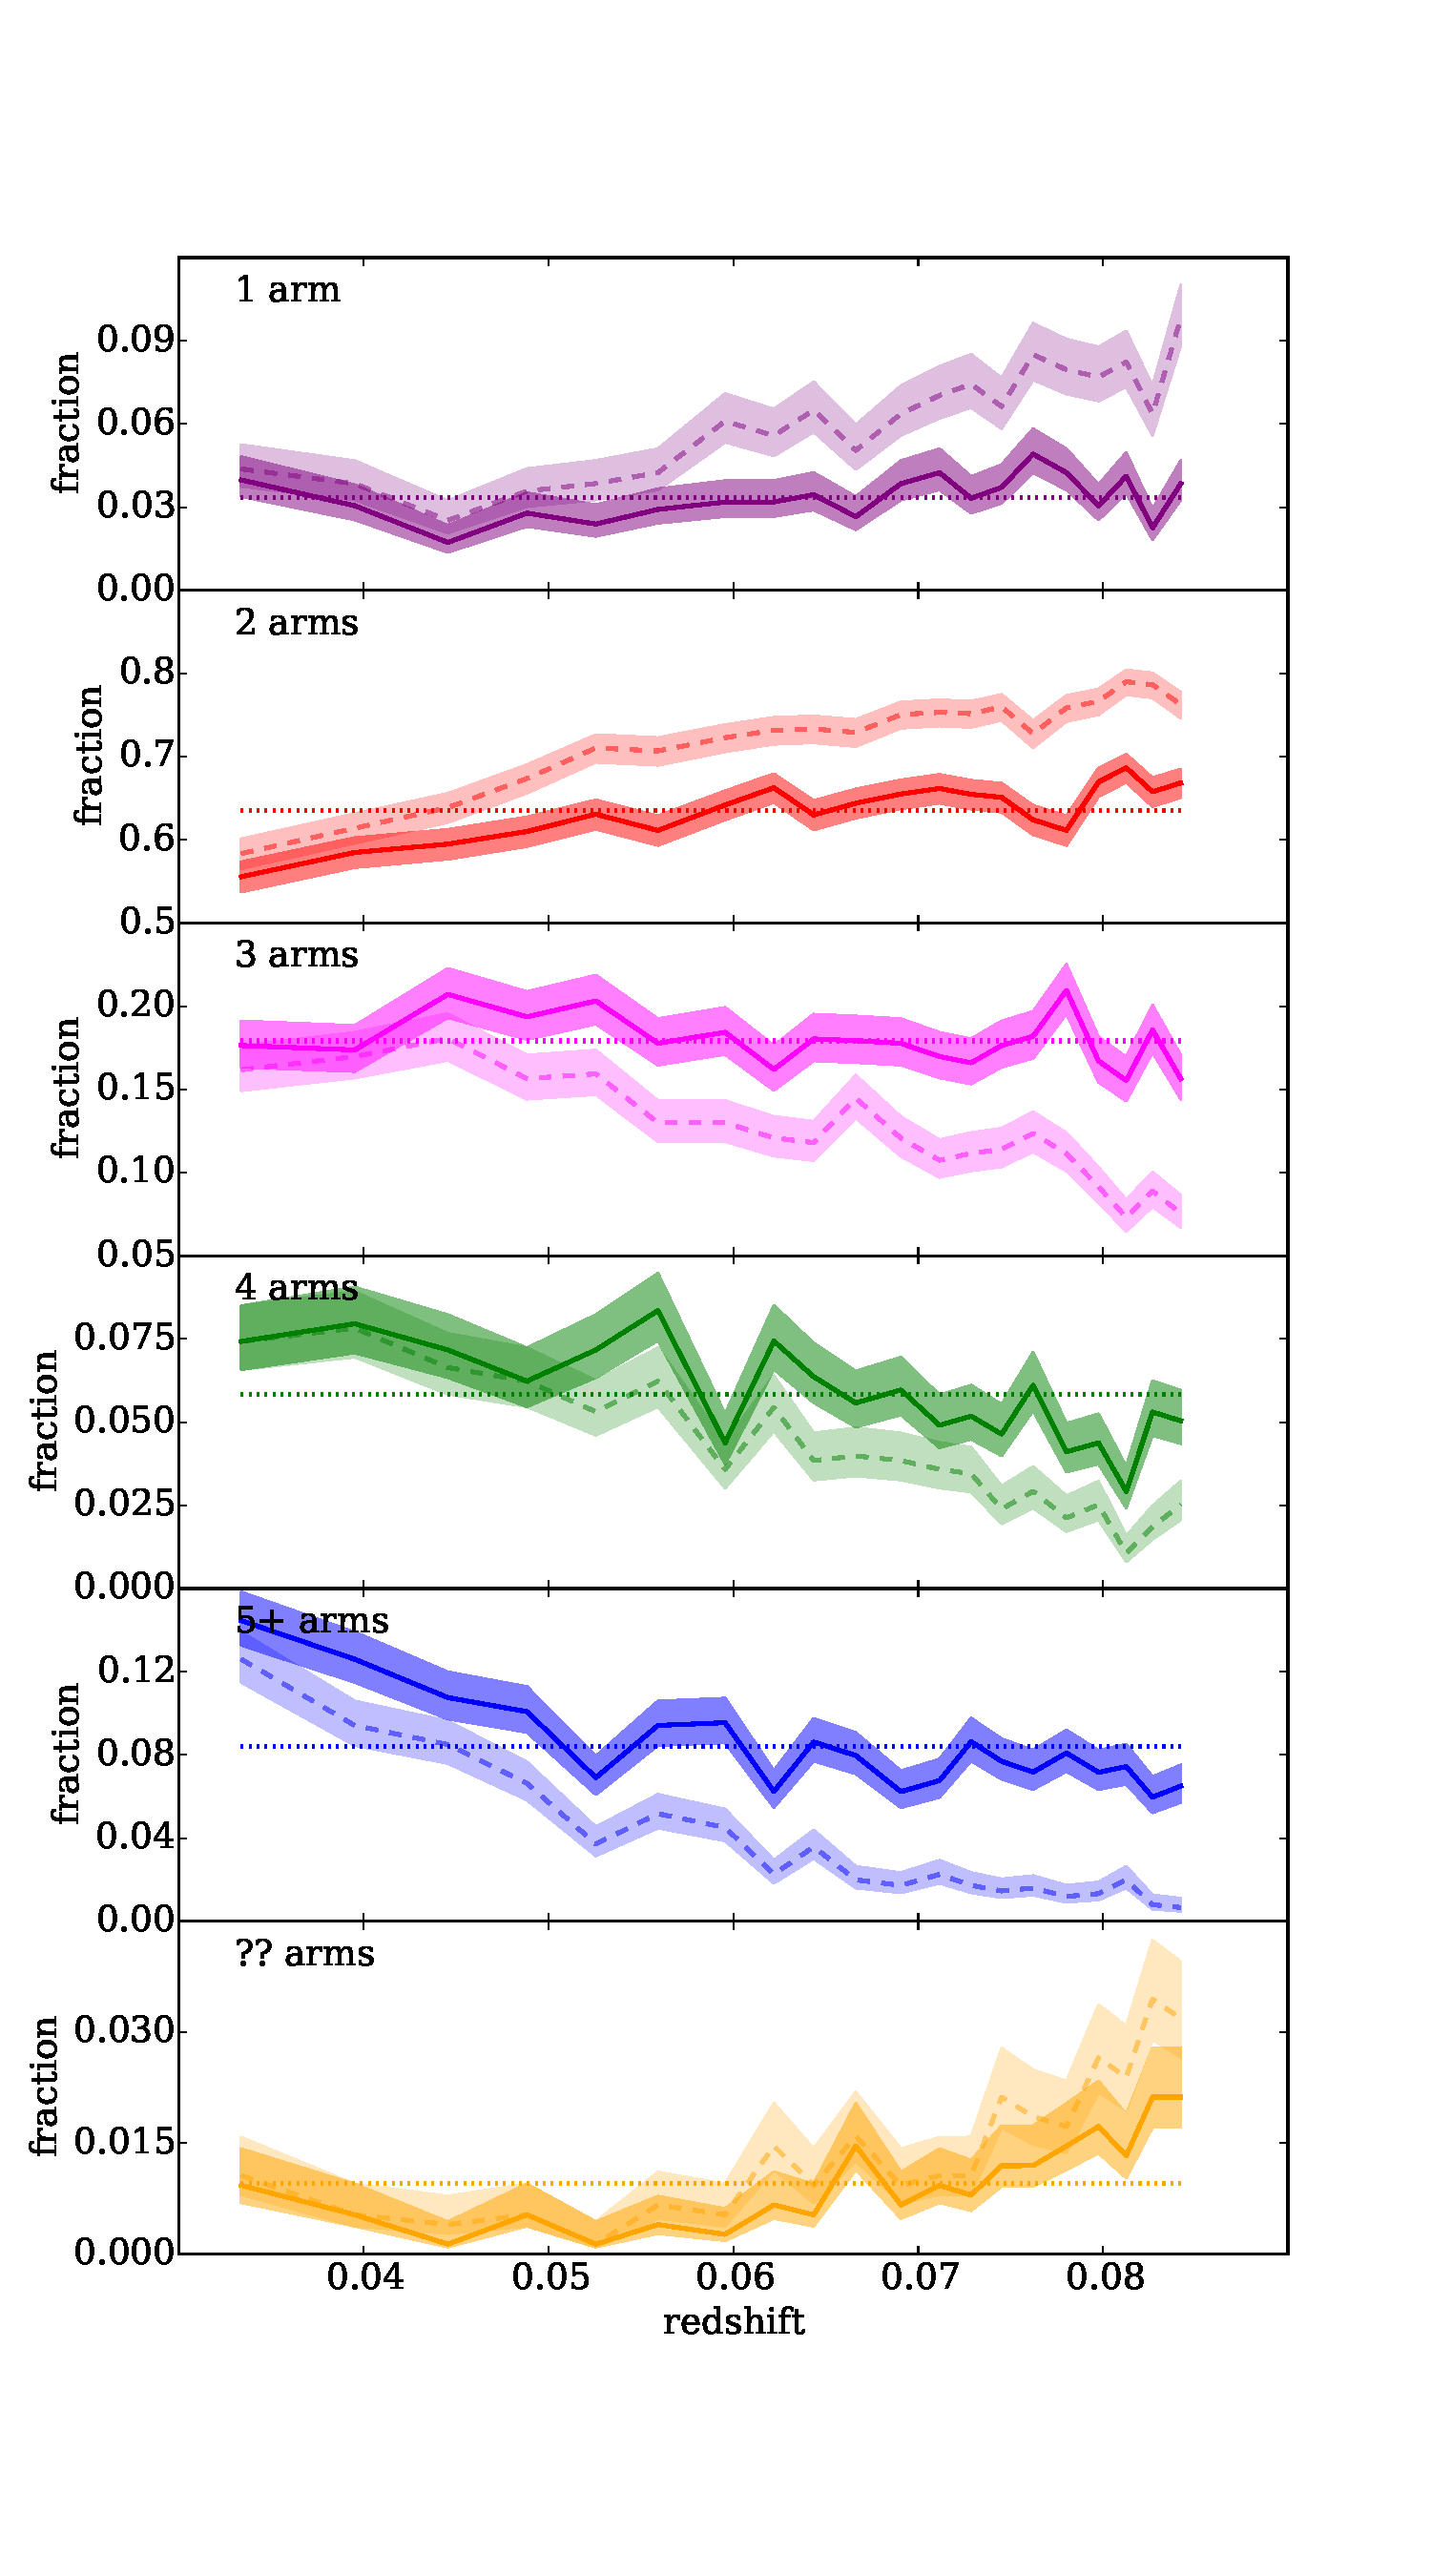
\includegraphics[width=0.5\textwidth]{Data_imgs/arm_number_with_z.pdf}
		
        \caption{Fraction of galaxies in the \textit{luminosity limited sample} classified as having 1,2,3,4, or more than 4 spiral arms as a function of redshift. The solid line indicates the debiased fractions, and the dashed line indicates the raw vote fractions. Errors are calculated using the method described in \citet{Cameron_11}.}
		
        \label{fig:arm_number_trend}
        
\end{figure}

An interesting question that has not been fully unexplored in GZ2 is the question of spiral arm multiplicity, or how many spiral arms galaxies have. The star forming properties have already been looked at using the vote fractions \citep{Willett_15}, but we wish to separate the galaxies in to separate populations to compare their properties.The new debiasing method is used to define a sample of galaxies that are classified as spiral galaxies with $p_{features} \times p_{not \, edge \, on} \times p_{spiral} > 0.5$. We also impose the cut of $N>5$, so that each of the galaxies has been observed by more than 5 people to make our selection less sensitive to noise. As a reference, samples selected in the same way using the original debiasing in \citet{Willett_13} are compared. galaxies are assigned to the spiral arm number by the highest value from the six possible answers to the spiral arm question. However, to maximise our galaxy samples, we also redistribute galaxies that have the highest debiased vote fraction for the 'can't tell' answer. The only limit that is applied is that we still include $N>5$ limit, but this time ignoring the 'can't tells'. All galaxies assigned as spirals in the \textit{luminosity limited sample} that have $>5$ individual classifications of arm number therefore make up our spiral sample. The fraction of galaxies with different arm numbers with respect to redshift are displayed in figure \ref{fig:arm_number_trend} and the overall properties of each of the populations are shown in table XX below. It can be seen from figure \ref{fig:arm_number_trend} that the new debiasing method means that samples are more complete in the higher redshift images. Figure XX shows a set of images at different redshifts classified as having either 1, 2, 3, 4 or more than 4 arms in different redshift bins. The basic properties of the galaxies in the spiral galaxy sample divided by spiral arm number are compared below.

\rh{'Image panel' of spiral galaxies to be put in here.}

\subsection{Stellar mass}
\label{sec:mass}

The distributions of stellar mass for each of the samples is shown in figure \ref{fig:mass_histogram}. From these plots, it is clear that there is no explicit dependence of arm number with stellar mass- each of the samples with different numbers of spiral arms spans the entire range of stellar mass from $10^{9} - 10^{11.5} M_{\odot}$. It must also be noted that the distributions in figure \ref{fig:mass_histogram} are of the \textit{volume-limited sample}, and are therefore incomplete for low stellar mass objects (see section \ref{sec:VLS}). If we only consider the distributions above this stellar mass limit, then the galaxy samples look very different. Galaxies with more spiral arms generally seem to have higher stellar masses. 

The trend with stellar mass can be clearly seen when plotting the fraction of spiral galaxies with 1,2,3,4 or more than 4 arms in bins of stellar mass, as shown in figure \ref{fig:mass_plot}. A clear trend is observed when looking at the highest stellar mass bins with $M_* \gtrsim 10^{11} M_{\odot}$. In the bins with lower stellar mass , the fraction of 2 and 5+ armed spiral galaxies remains consistent. However, a significant increase in galaxies with more than 4 spiral arms is observed with the most massive spiral galaxies with $M_* \gtrsim 10^{11} M_{\odot}$. In the bin of $M_* = 10^{11.97}M_{\odot}$, only $4 \pm 1 \%$ of galaxies are observed to have more than 4 spiral arms compared with $54 \pm 3 \%$ of the galaxies having 2 spiral arms. However, in the highest mass bin with $M_* = 10^{11.21}M_{\odot}$, a significant increase is seen in the fraction of 5+ armed spiral galaxies, with $15 \pm 2 \%$ of the galaxies have more than 4 spiral arms compared with $44 \pm 3 \%$ galaxies having 2 spiral arms.

\begin{figure*}
		\centering
		
        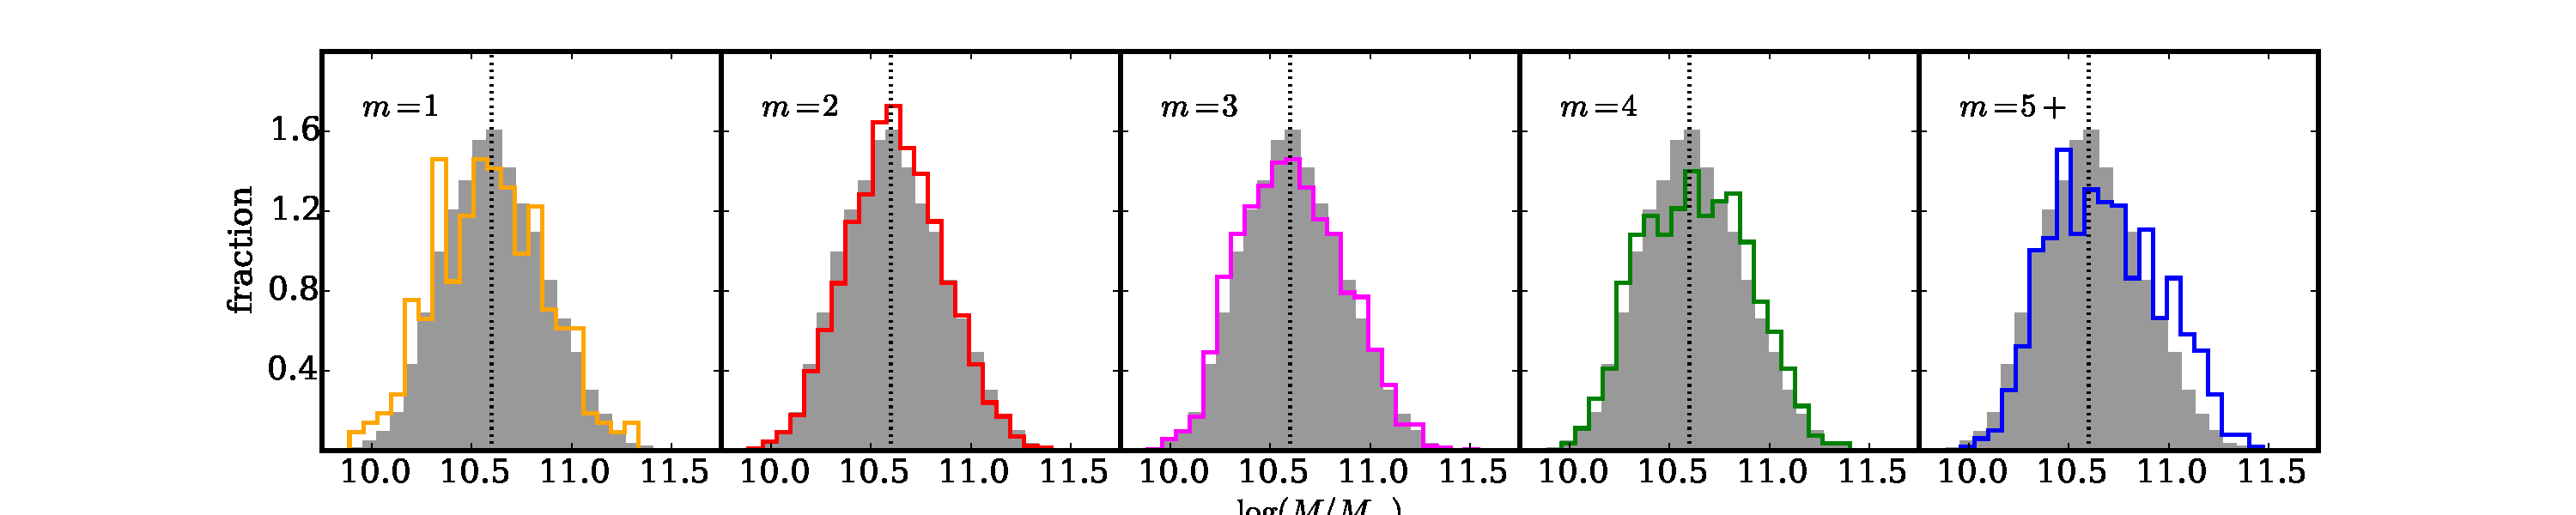
\includegraphics[width=1\textwidth]{Results_imgs/mass_histogram.pdf}
		
        \caption{Stellar mass distributions for each arm number subsample. The stepped histograms show the distributions for each of the \textit{arm number subsamples}, and the filled grey histograms show the distribution for all of the spiral galaxies in the \textit{volume limited sample}. The dotted line shows the lower limit to the \textit{stellar mass limited sample}.}
		
        \label{fig:mass_histogram}
        
\end{figure*}

\begin{figure}
		\centering
		
        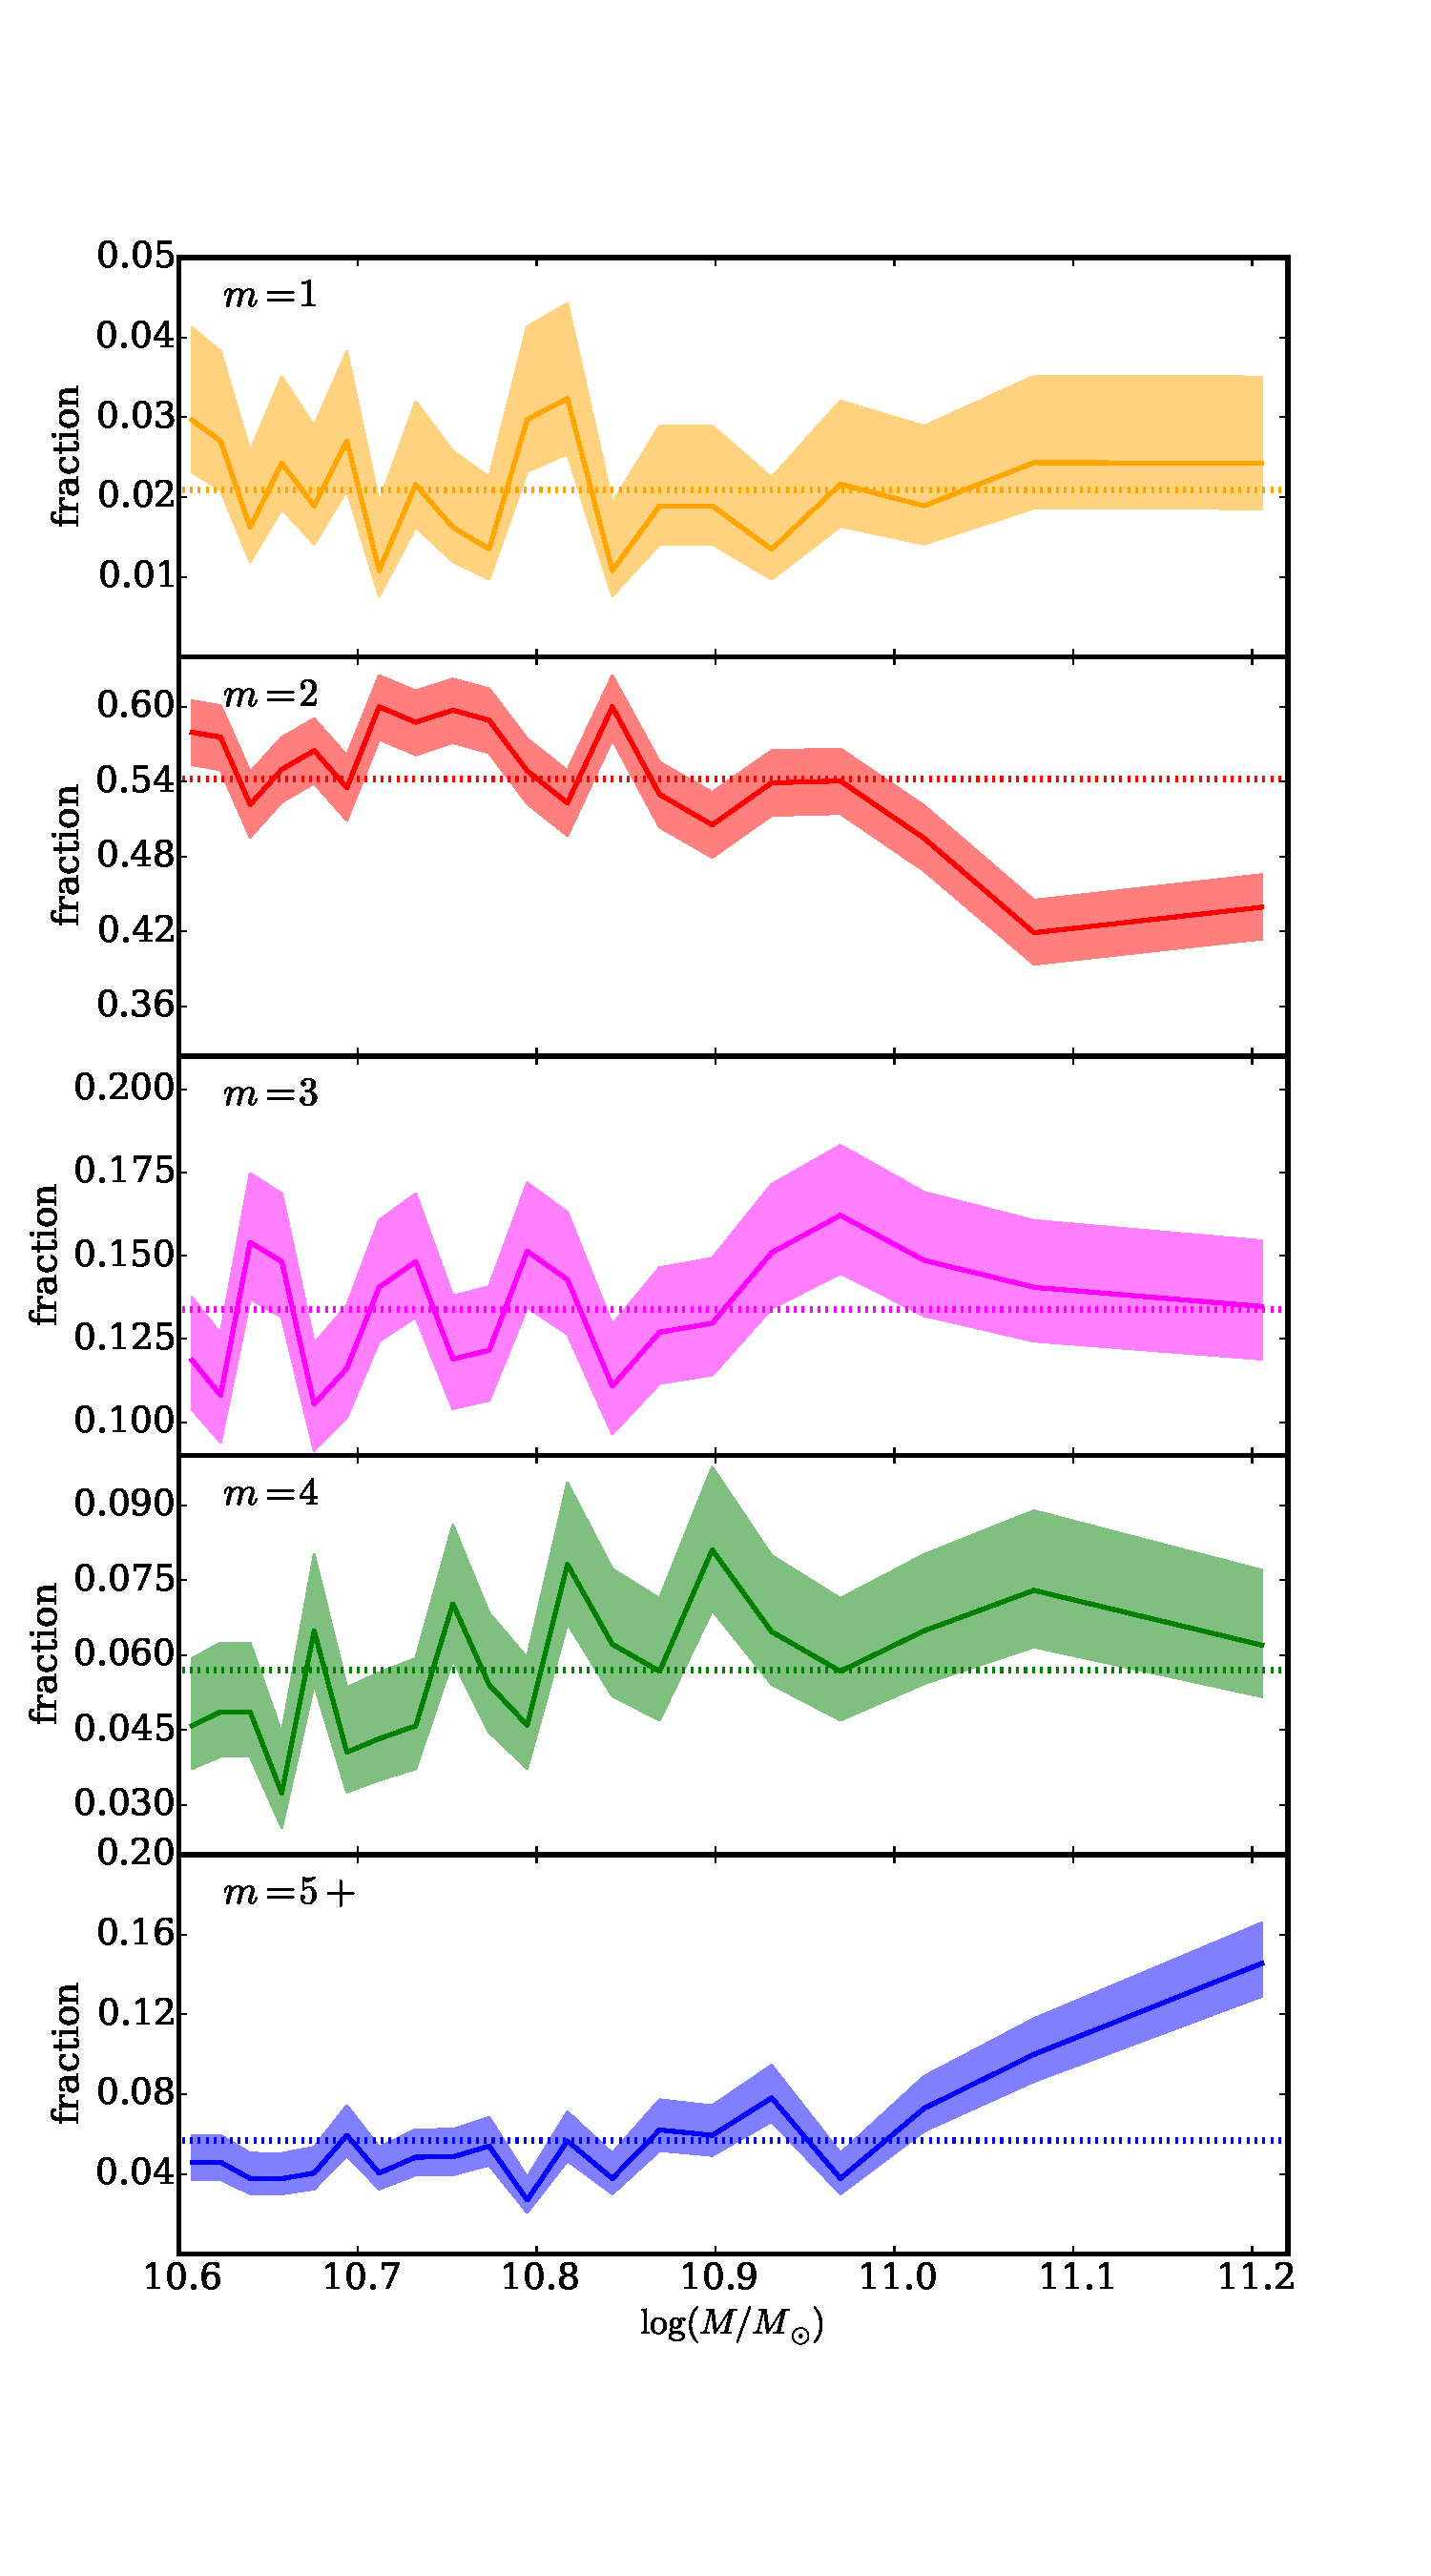
\includegraphics[width=0.5\textwidth]{Results_imgs/mass_plot.pdf}
		
        \caption{Fraction of galaxies with $m$ spiral arms for the stellar mass limited spiral sample, binned by stellar mass. The shaded region indicates the $\pm 1 \sigma$ error calculated using the method described in \protect\cite{Cameron_11}.}
		
        \label{fig:mass_plot}
        
\end{figure}

%------------------------------------------------------------------------------------

\subsection{Galaxy colours}

\begin{figure*}
		\centering
		
        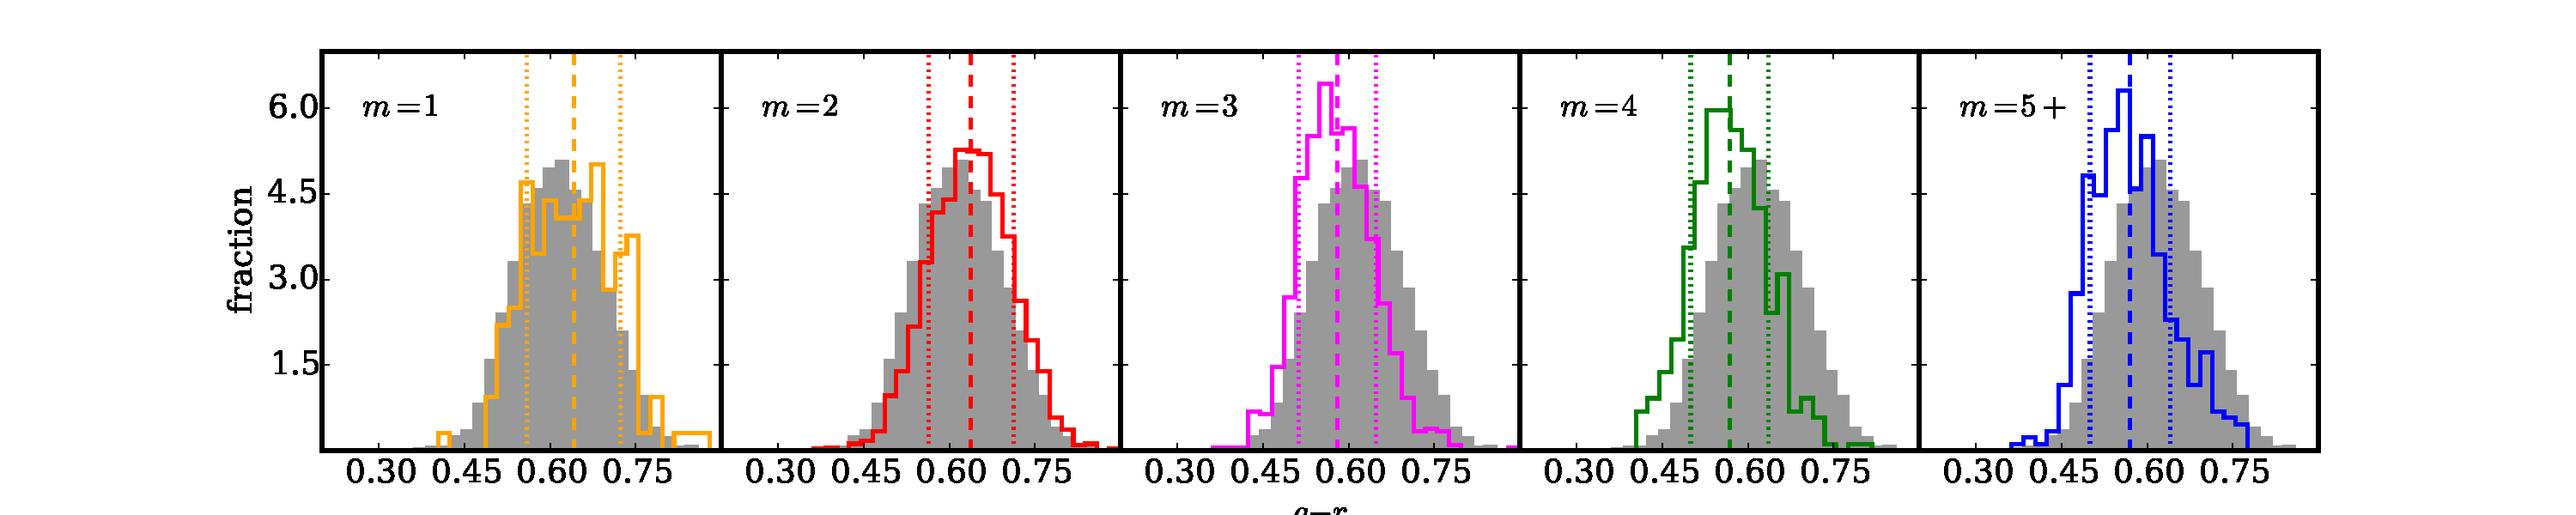
\includegraphics[width=1\textwidth]{Results_imgs/colour_histogram.pdf}
		
        \caption{$g-r$ colours for each of the galaxy \textit{arm number samples}. The grey distribution shows the total spiral sample in the \textit{stellar mass limited samples}. The dashed vertical lines indicate the mean $g-r$ colours of each of the \textit{arm number samples}, and the dotted vertical lines indicate the standard deviation of each of the samples.}
		
        \label{fig:colour_histogram}
        
\end{figure*}

The galaxy samples are also compared in terms of colour, in order to give an insight in to the star-formation properties of each of the samples. Bluer colours are generally associated with more recent star formation and therefore younger stellar populations. It is also well known that galaxy colour correlates with stellar mass, with more massive galaxies being redder in colour \citep{Baldry_06}, so the \textit{stellar mass limited sample} is used for this analysis to ensure completeness. The distributions for each of the \textit{arm number samples} are shown in figure \ref{fig:colour_histogram}. The distributions show that there is a marked difference in the colours of the galaxies with many spiral arms, compared to the 2 armed galaxy population. The 2 armed spiral sample has a mean $g-r$ colour of 0.64 and a standard deviation of 0.07. Comparatively, the 4 and 5+ armed spirals both have a mean $g-r$ colour of 0.57 and a standard deviation of 0.07. For comparison, the standard deviation of the entire spiral sample is 0.08, so the associated shift colour shift between 2 armed and 4 or 5+ armed spirals corresponds to $\sim 1 \sigma$. This result is perhaps surprising, as these galaxies have greater stellar mass, which would normally mean that such galaxies are redder in colour. The result therefore indicates that the stellar populations of many armed spiral galaxies are much younger than the stellar populations in 2 armed spiral galaxies. 

\begin{figure}
		\centering
		
        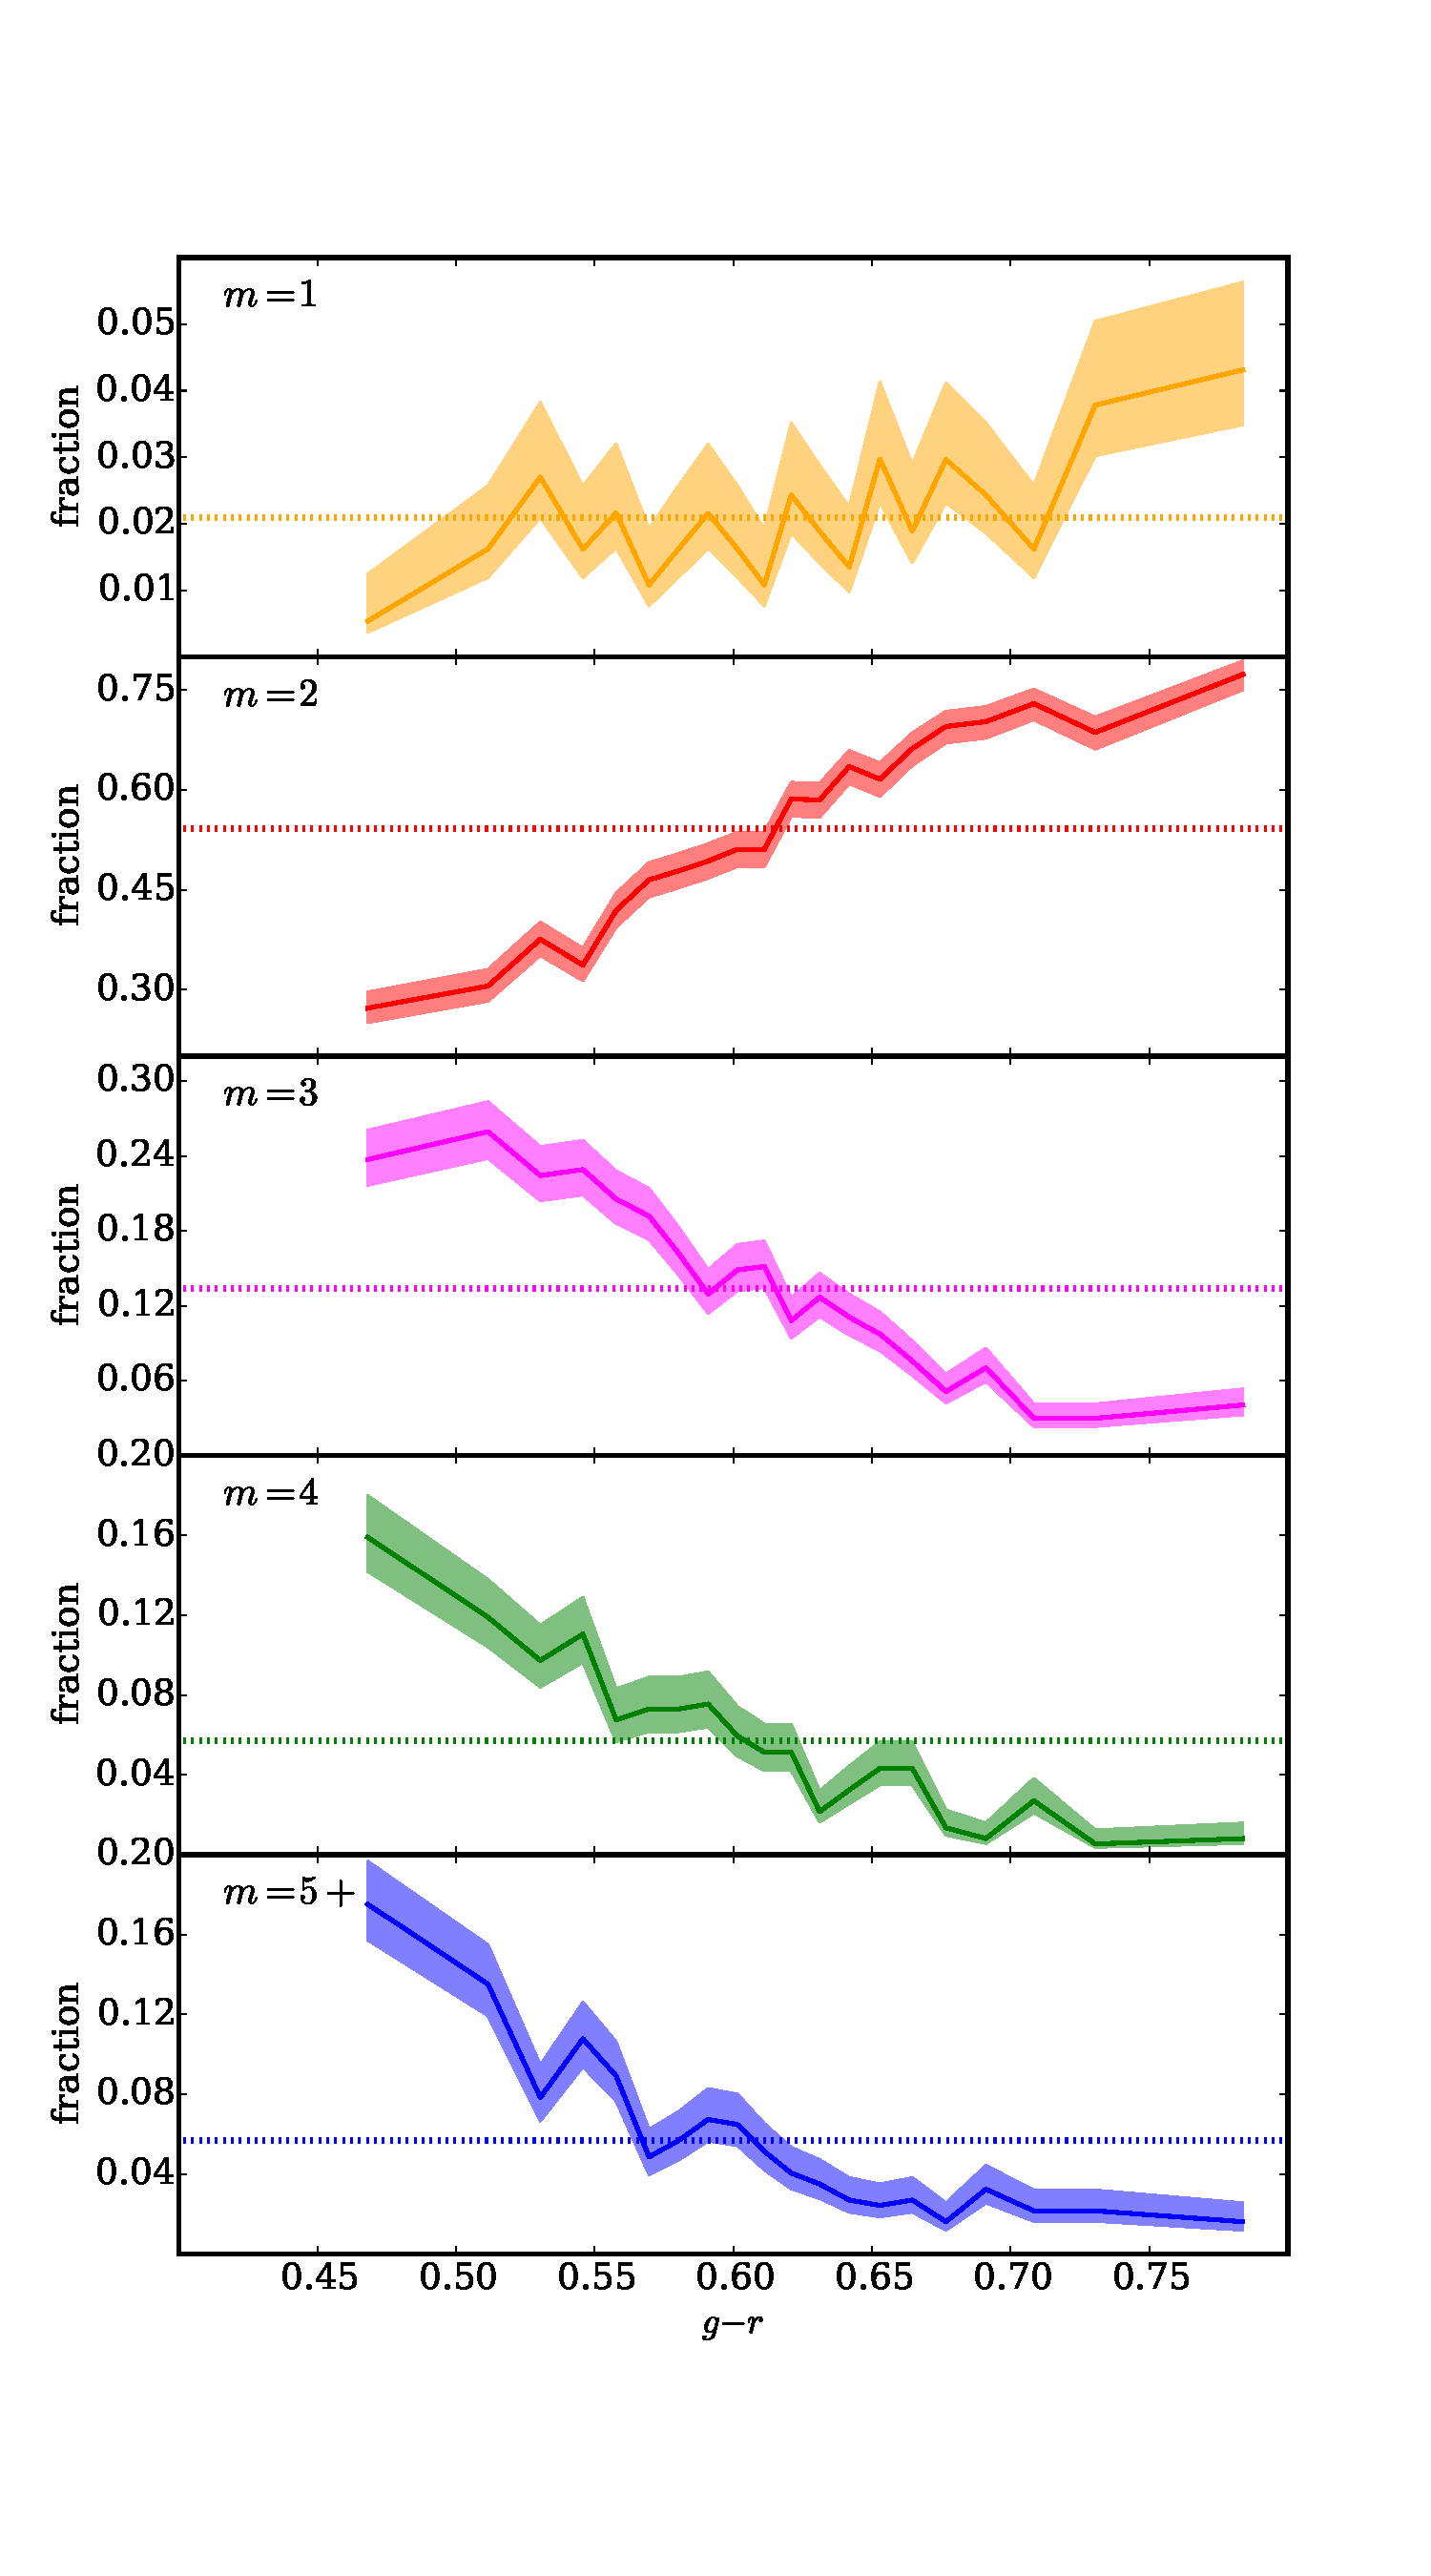
\includegraphics[width=0.5\textwidth]{Results_imgs/colour_plot.pdf}
		
        \caption{Fraction of galaxies with 1,2,3,4 or more than 4 arms binned by $g-r$ colour. The dotted line shows the mean fraction averaged over all of the bins for each of the samples, and the shaded region show the $1 \sigma$ errors.}
		
        \label{fig:colour_plot}
        
\end{figure}

The fraction of spirals with different numbers of spiral arms can also be compared by binning the data by colour, and the results are shown in figure \ref{fig:colour_plot}. The trends with colour also seem to be much stronger than those observed with stellar mass in section \ref{sec:mass}, with all  samples with the exception of the 1 armed galaxy sample showing a clear positive or negative correlation with colour. For the reddest population of galaxies, with $g-r=0.78$, the sample is dominated by grand design spiral structure, with $77 \pm 2 \%$ of the galaxies in that bin having 2 spiral arms. Conversely, in the bluest bin, with $g-r=0.47$, only $27 \pm 2 \%$ display 2 armed structure. The galaxies at the bluest end of the spectrum are dominated by galaxies with 3,4 or more than 4 spiral arms, with $57 \pm 3 \%$ of the galaxies in the bluest bin having 3,4 or more than 4 spiral arms compared to $6 \pm 1 \%$ in the bin containing the reddest spiral galaxies. 

%------------------------------------------------------------------------------------

\subsubsection{Star formation rates}
\label{sec:SFR}

The bluer colours of the many-armed spiral galaxies could be indicative of a higher star formation rate. We therefore plot the specific star formation rate distributions for each of spiral arm subsamples in figure XX. The distributions show that the bluer colours of the many armed spiral samples is not due to an enhanced star formation rate- the peaks of the distributions is not at a significantly higher value of sSFR. The main differences between the distributions are actually at the very highest and lowest ends of the sSFR scales. The 2 and more than 4 armed galaxies have an extended tail of low-sSFR galaxies that is not observed in the 3 and 4 armed galaxy distributions. The more than 4 armed distribution also shows that more than 4 armed galaxies do not have a significant fraction of galaxies with the very highest sSFRs, with the distribution seeming to have a maximimum value of $\sim 10^{-10} M_{\odot} yr^{-1}M_*^{-1}$. The only sample with a population of significantly enhanced sSFRs is the 1 armed galaxy sample. 

\begin{figure*}
		\centering
		
        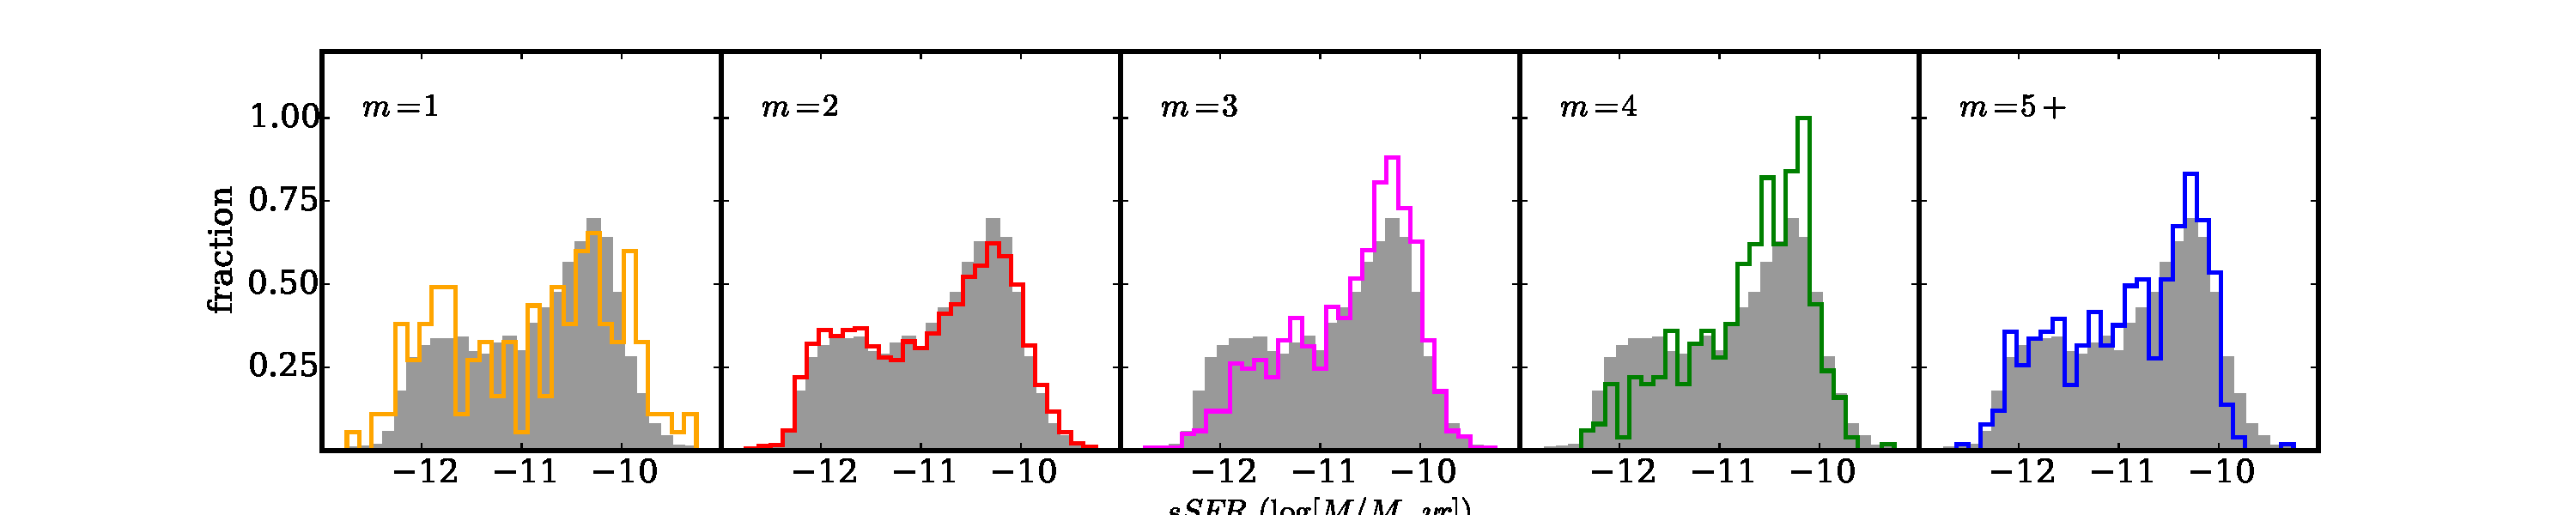
\includegraphics[width=1\textwidth]{Results_imgs/ssfr_histogram.pdf}
		
        \caption{Distribution of sSFRs for each of the arm number subsamples. The stepped histograms show each of the subsamples and the grey shaded histogram shows the total spiral sample.}
		
        \label{fig:ssfr_histogram}
        
\end{figure*}

%------------------------------------------------------------------------------------
\subsection{Colour vs. stellar mass}
\label{sec:colour_mass}

Having demonstrated that the different galaxy populations have different stellar mass and colour properties, we now look in to these differences in more detail. The colour-mass contour is plotted in figure \ref{fig:cm1}, to check what the colour offset is with respect to stellar mass. The plots show that for a given stellar mass, the 3,4 and more than 4 armed galaxies are systematically bluer in the $g-r$ colour band. How much offset is observed for a given stellar mass is considered by fitting a best fit line to the data. The gradient of the line is set as constant using the entire \textit{stellar mass-limited spiral sample}. The calculated offsets indicate that for a given stellar mass, the 3 armed galaxy has a $g-r$ colour 0.06 lower than the 2 armed galaxy sample. The offsets in the 4 and 5+ armed samples are higher, with values of 0.07 and 0.08 respectively.

\begin{figure}
		\centering
		
        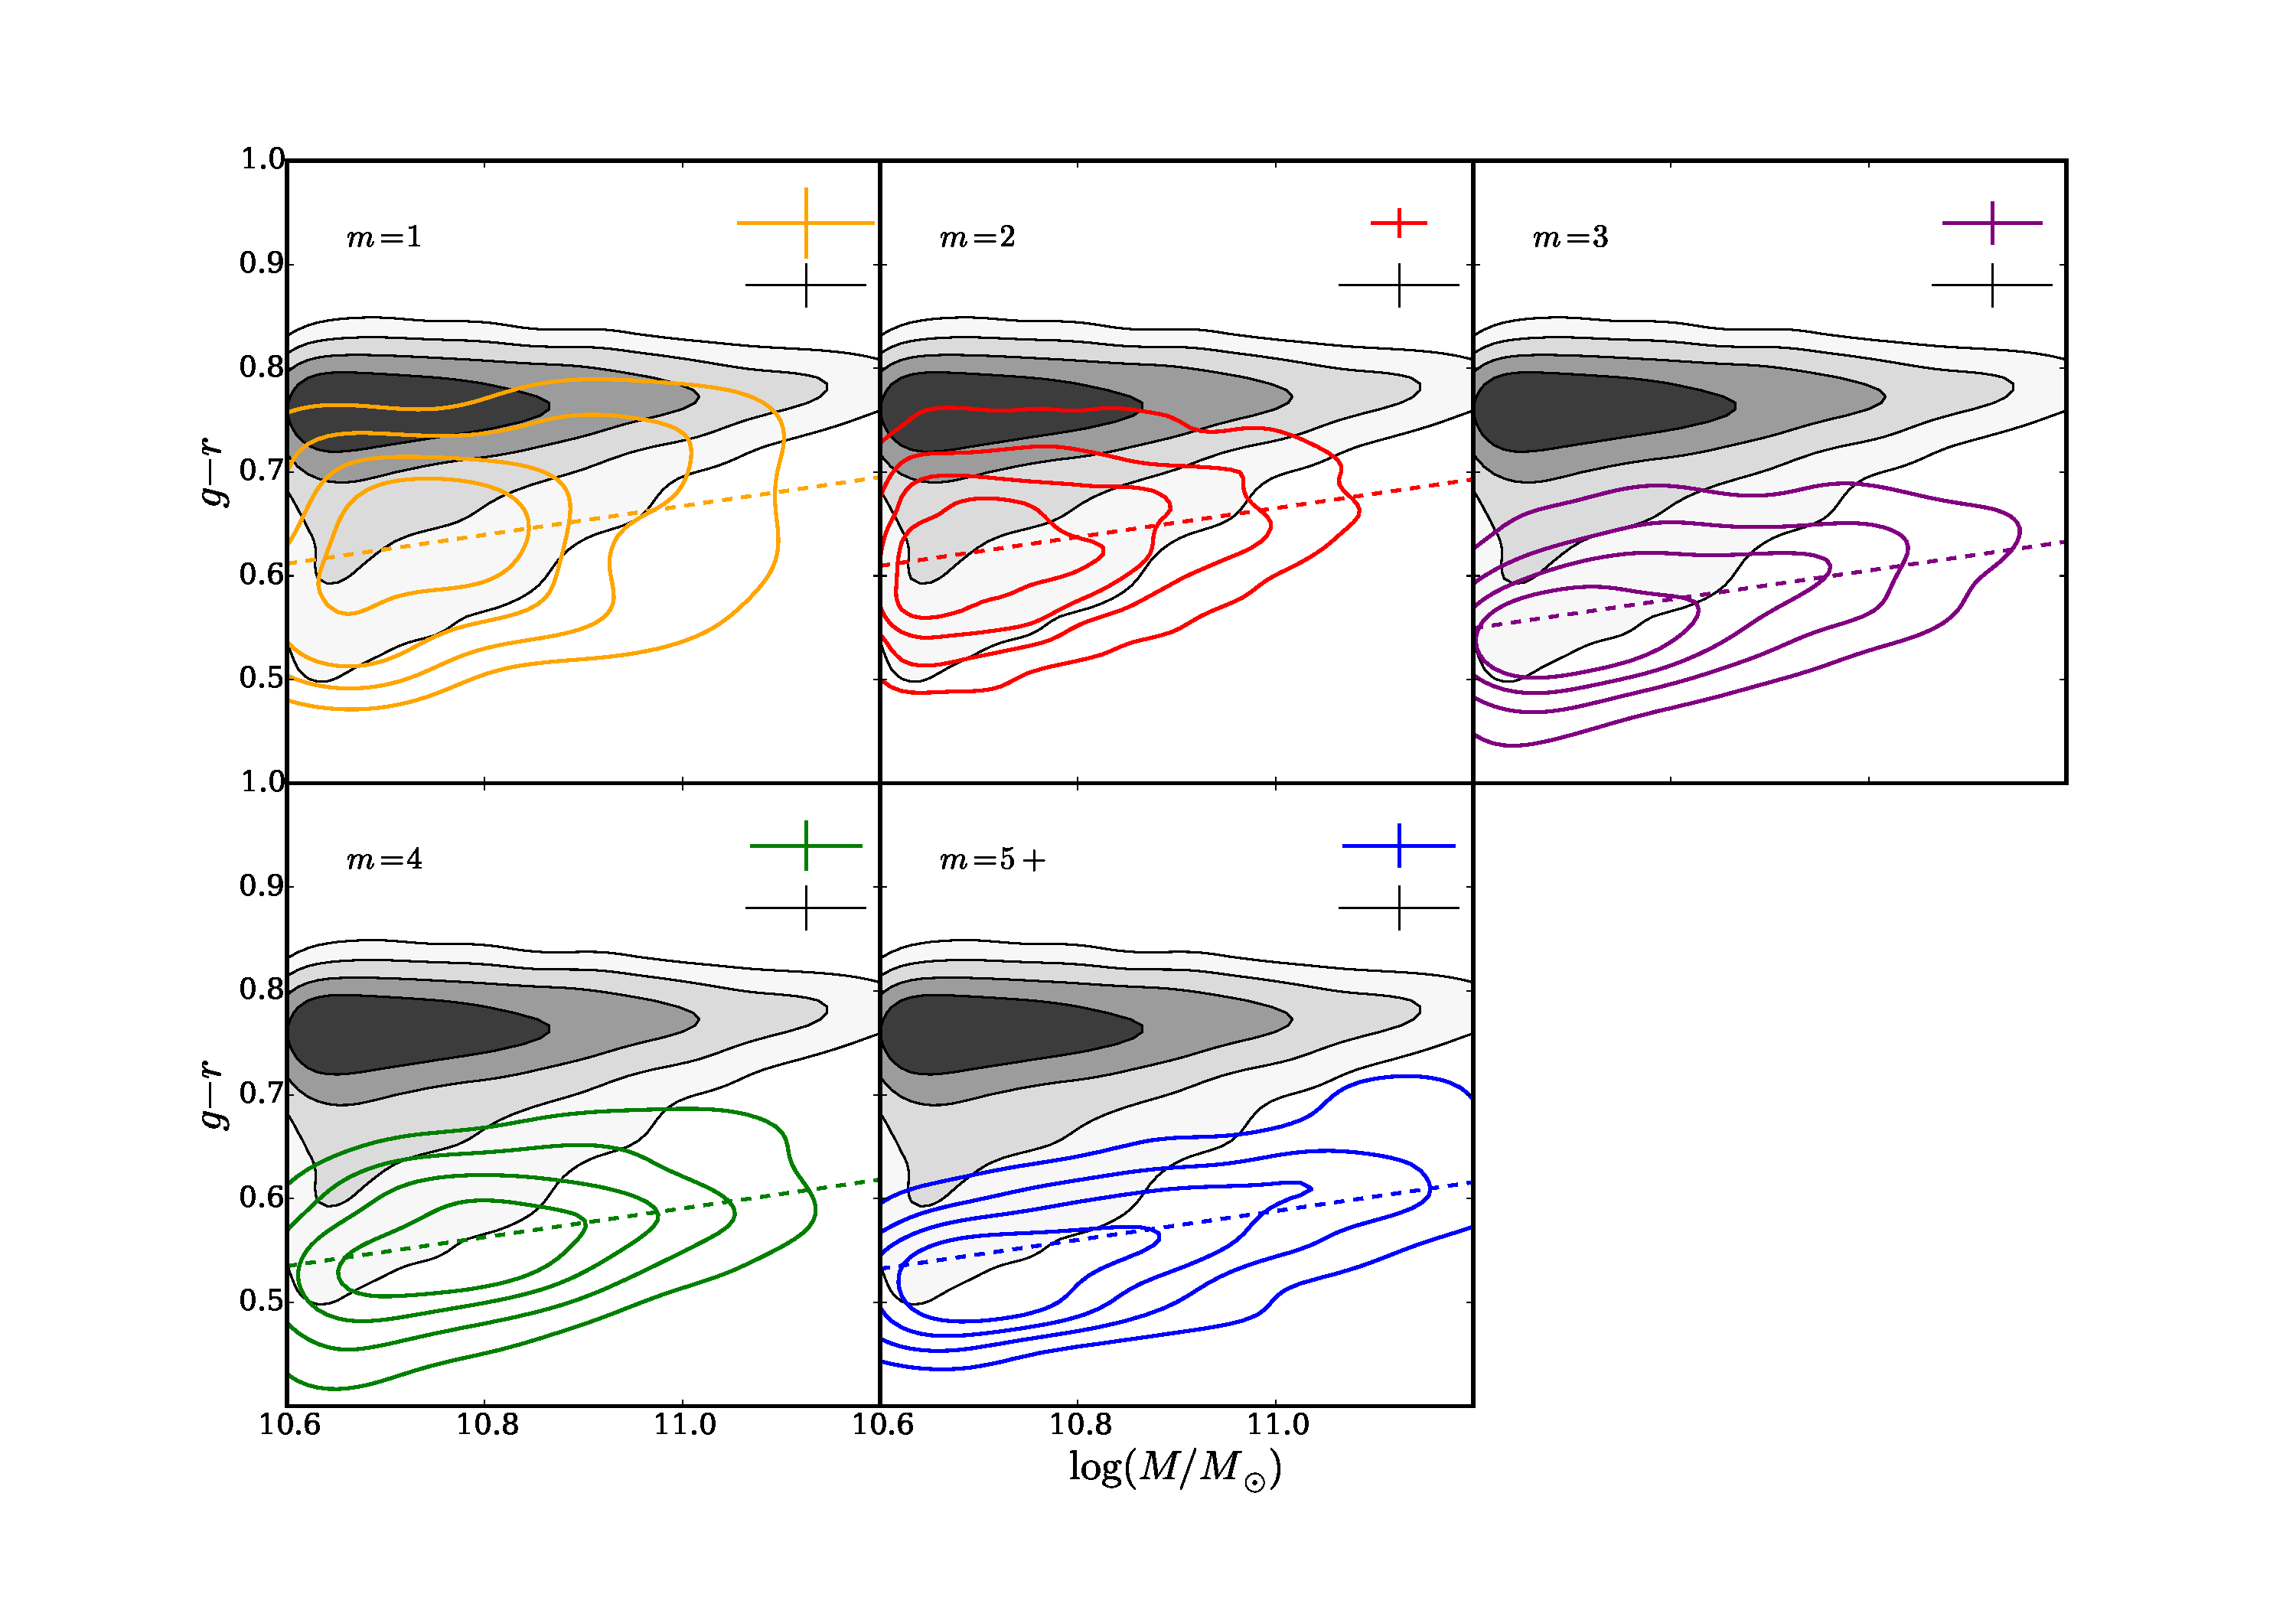
\includegraphics[width=0.5\textwidth]{Results_imgs/colour_mass_1.pdf}
		
        \caption{$g-r$ vs stellar mass for each of the \textit{stellar mass-limited arm number samples}. The grey filled contour indicates the full stellar mass limited sample. The contour lines extending outwards indicate the area enclosing 20,40,60 and 80\% of each sample. Each contour shows a kernel density estimate (KDE), optimised using 5-fold cross validation. The optimised bandwidths are indicated with the crosses in the top right-hand side of each figure. The dotted lines indicate the best fit line to the data, with a constant gradient of 0.14 set by the \textit{stellar mass-limited spiral sample}.}
		
        \label{fig:cm1}
        
\end{figure}
%------------------------------------------------------------------------------------
%%%%%%%%%%%%%%%%%%%%%%%%%%%%%%%%%%%%%%%%%%%%%%%%%%%%%%%%%%%%%%%%%%%%%%%%%%%%%%%%%%%%%
%------------------------------------------------------------------------------------
\section{Conclusions}
\label{sec:conclusions}

An examination of the properties of spiral galaxies with respect to their disk structure is presented using statistical morphological data from Galaxy Zoo. We show that employing a new debiasing procedure allows us to compare the properties of a spectroscopically complete sample of XX galaxies, of which XX can be classified as spirals and compared in terms of spiral arm number. Using this new debiasing method, clear differences in the overall properties of spiral galaxies are observed. By defining a stellar mass limited sample of spiral galaxies, it is seen that galaxies with greater numbers of spiral arms have higher stellar masses \rh{(Numbers?)}. A clear trend is also observed with respect to galaxy colour, with 4 and more than 4 armed spiral galaxies being much bluer in the $g-r$ colour band. The most stark contrast is observed when comparing the 2 armed spiral galaxy population with the more than 4 armed spiral galaxy population- we observe that for a given stellar mass, more than 4 armed spiral galaxies are $XX \pm XX$ bluer in $g-r$ than 2 armed spiral galaxies. However, there is no significant difference observed in the star formation rates of galaxies with different numbers of spiral arms. This suggests  that the $g-r$ colour differences are not attributable to more recent star formation in more than 4 armed spiral galaxies, and may therefore be due to 2 armed spiral galaxies having an older overall stellar population, or containing more dust.  

%------------------------------------------------------------------------------------
%%%%%%%%%%%%%%%%%%%%%%%%%%%%%%%%%%%%%%%%%%%%%%%%%%%%%%%%%%%%%%%%%%%%%%%%%%%%%%%%%%%%%
%------------------------------------------------------------------------------------

\section{Acknowledgements}

The data in this paper are the result of the efforts of the Galaxy Zoo 2 volunteers, without whom none of this work would be possible. Their efforts are individually acknowledged at authors.galaxyzoo.org. I'd also like to acknowledge my man Steven for being a legend.


\bibliographystyle{mn2e}
\bibliography{jun15}

\end{document}